% \ll --> compile
% \lv --> view

\documentclass[a4paper]{article}
%-----------------------------
% preamble
%-----------------------------
\usepackage[sumlimits,]{amsmath}
\usepackage[utf8]{inputenc}
\usepackage[english]{babel}
\usepackage{graphicx}
\usepackage{subcaption}
\usepackage{hyperref}
%\usepackage[document]{ragged2e}

\graphicspath{ 
    {../figures/} 
    {../figures/theoretical-ex/} 
    {../figures/pre-ex1/} 
    {../figures/pre-ex2/} 
    {../figures/ex1/} 
    {../figures/ex2/} 
}

%-----------------------------
% body
%-----------------------------
\begin{document}

% UNICAMP logo
\begin{figure}[t]
    \centering
    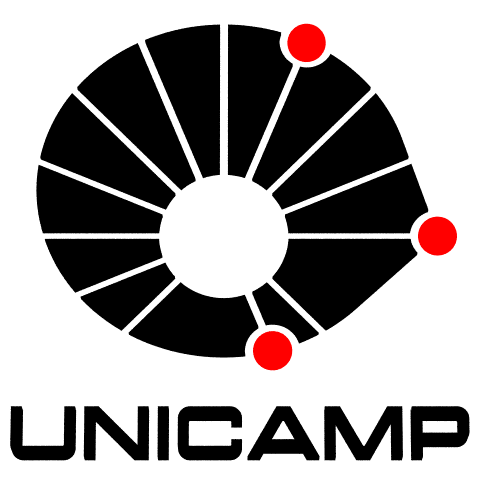
\includegraphics[width=1.5cm]{unicamp}
    \label{fig:unicamp}
\end{figure}

% FEEC logo
\begin{figure}[t]
    \centering
    
\includegraphics[width=1.5cm]{feec}
    \label{fig:feec}
\end{figure}

\title{EFC1 - Exercise 1}
\author{Rafael Claro Ito}
%R.A.: 118430
%ito.rafael@gmail.com
\date{September 2019}
\maketitle
\newpage

%-----------------------------
%\listoffigures
%-----------------------------



%-----------------------------
% Abstract
%-----------------------------
%\begin{abstract}
%    ...Your abstract goes here...
%\end{abstract}
%-----------------------------
% Sectioning
%-----------------------------
%\chapter{Introduction}
%This chapter's content...
%
%\section{Structure}
%This section's content...
%
%\subsection{Top Matter}
%This subsection's content...
%
%\subsubsection{Article Information}
%This subsubsection's content...
%-----------------------------


%=================================================
\section{Theoretical Activites}
%=================================================

%=======================================
\subsection{Exercise 1}
%=======================================

%==============================
\subsubsection{a) Obtenha P(X) e P(Y).}
%==============================

%------------------------
% P_X(0)
\paragraph{$i) \; P_X(0):                       $
\\
$ \displaystyle P_X(0) = \sum_{y} P_{XY}(0,y)   $\\
$ P_X(0) = P_{XY}(0,0) + P_{XY}(0,1)            $\\
$ P_X(0) = 1/6 + 3/8                            $\\
$ \boxed{ P_X(0) = 13/24 }                      $\\
}
%------------------------
% P_X(1)
\paragraph{$ii) \; P_X(1):                      $
\\
$ \displaystyle P_X(1) = \sum_{y} P_{XY}(1,y)   $\\
$ P_X(1) = P_{XY}(1,0) + P_{XY}(1,1)            $\\
$ P_X(1) = 1/8 + 1/3                            $\\
$ \boxed{ P_X(1) = 11/24 }                      $\\
}
%------------------------
% P_Y(0)
\paragraph{$iii) \; P_Y(0):                     $
\\
$ \displaystyle P_Y(0) = \sum_{y} P_{XY}(x,0)   $\\
$ P_Y(0) = P_{XY}(0,0) + P_{XY}(1,0)            $\\
$ P_Y(0) = 1/6 + 1/8                            $\\
$ \boxed{ P_Y(0) = 7/24 }                       $\\
}
%------------------------
% P_Y(1)
\paragraph{$iv) \; P_Y(1):                      $
\\
$ \displaystyle P_Y(1) = \sum_{y} P_{XY}(x,1)   $\\
$ P_Y(1) = P_{XY}(0,1) + P_{XY}(1,1)            $\\
$ P_Y(1) = 3/8 + 1/3                            $\\
$ \boxed{ P_Y(1) = 17/24 }                      $\\
}

%==============================
\subsubsection{b) Calcule P(X = 0|Y = 0).}
%==============================
% P(X=0|Y=0)
\paragraph{
$ \displaystyle P_{X|Y}(x,y) = \frac{P_{XY}(x,y)}{P_Y(y)}   $\\
$ \displaystyle P_{X|Y}(0,0) = \frac{P_{XY}(0,0)}{P_Y(0)}   $\\
$ P_{X|Y}(0,0) = \frac{1/6}{7/24}                           $\\
$ \boxed{ P_{X|Y}(0,0) = 4/7 }                              $\\
}

%==============================
\subsubsection{c) Calcule E[X] e E[Y].}
%==============================

%------------------------
% E[X]
\paragraph{$ i) \; E[X]:                       $
\\
$ \displaystyle E[X] = \sum_{k} x_k P_X(x_k)   $\\
$ E[X] = 0 \cdot P_X(0) + 1 \cdot P_X(1)       $\\
$ \boxed{ E[X] = 11/24 }                       $\\
}
%------------------------
% E[Y]
\paragraph{$ ii) \; E[Y]:                      $
\\
$ \displaystyle E[Y] = \sum_{k} y_k P_Y(y_k)   $\\
$ E[Y] = 0 \cdot P_Y(0) + 1 \cdot P_Y(1)       $\\
$ \boxed{ E[Y] = 17/24 }                       $\\
}

%==============================
\subsubsection{d) As variáveis são independentes? Por quê?}
%==============================
%\\
%\\
%\\
TO BE WRITTEN
%\\
%\\
%\\

%=======================================
\subsection{Exercise 2}
%=======================================

%==============================
\subsubsection{a) Calcule H(X), H(Y) e H(X|Y).}
%==============================

$ P_X(0) = P_{XY}(0,0) + P_{XY}(0,1) = 1/4     $
$ P_X(1) = P_{XY}(1,0) + P_{XY}(1,1) = 3/4     $
$ P_Y(0) = P_{XY}(0,0) + P_{XY}(1,0) = 3/8     $
$ P_Y(1) = P_{XY}(0,1) + P_{XY}(1,1) = 5/8     $

%------------------------
% H(X)
\paragraph{$ i) \; H(X):                                    $
\\
$ \displaystyle H(X) = -\sum_{x} p(x) \log_2 [p(x)]         $\\
$ H(X) = -P_X(0) \log_2 [P_X(0)] -P_X(1) \log_2 [P_X(1)]    $\\
$ \displaystyle 
    H(X) = - \frac{1}{4} \log_2 \left( \frac{1}{4} \right) 
           - \frac{3}{4} \log_2 \left( \frac{3}{4} \right)  $\\
$ H(X) = 0.5 + 0.3113                                       $\\
$ \boxed{ H(X) = 0.8113 }                                   $\\
}
%------------------------
% H(Y)
\paragraph{$ ii) \; H(Y):                                   $
\\
$ \displaystyle H(Y) = -\sum_{y} p(y) \log_2 [p(y)]         $\\
$ H(Y) = -P_Y(0) \log_2 [P_Y(0)] -P_Y(1) \log_2 [P_Y(1)]    $\\
$ \displaystyle 
    H(Y) = - \frac{3}{8} \log_2 \left( \frac{3}{8} \right) 
           - \frac{5}{8} \log_2 \left( \frac{5}{8} \right)  $\\
$ H(Y) = 0.5306 + 0.4238                                    $\\
$ \boxed{ H(Y) = 0.9544 }                                   $\\
}
%------------------------
% H(X,Y)
\paragraph{$ iii) \; H(X,Y):                                $
\\
$ \displaystyle 
    H(Y) = -\sum_x \sum_y p(x,y) \log_2 [p(x,y)]            $\\
$ H(Y) = - P_{XY}(0,0) \log_2 [P_{XY}(0,0)]                
         - P_{XY}(0,1) \log_2 [P_{XY}(0,1)] 
         - P_{XY}(1,0) \log_2 [P_{XY}(1,0)] 
         - P_{XY}(1,1) \log_2 [P_{XY}(1,1)]                 $\\
$ \displaystyle
    H(Y) = - 0 \cdot \log_2 (0)                              
          - \frac{1}{4} \log_2 \left( \frac{1}{4} \right)
          - \frac{3}{8} \log_2 \left( \frac{3}{8} \right)
          - \frac{3}{8} \log_2 \left( \frac{3}{8} \right)   $\\
$ H(Y) = 0 + 0.5 + 0.5306 + 0.5306                          $\\
$ \boxed{ H(Y) = 1.5613 }                                   $\\
}

%==============================
\subsubsection{b) Calcule H(X|Y) e H(Y|X).}
%==============================

%------------------------
% H(X|Y)
\paragraph{$ i) \; H(X|Y):      $
\\
$ H(X,Y) = H(Y) + H(X|Y)        $\\
$ H(X|Y) = H(X|Y) - H(Y)        $\\
$ H(X|Y) = 1.5613 - 0.9544      $\\
$ \boxed{ H(X|Y) = 0.6068 }     $\\
}
%------------------------
% H(Y|X)
\paragraph{$ ii) \; H(Y|X):     $
\\
$ H(X,Y) = H(X) + H(Y|X)        $\\
$ H(Y|X) = H(X,Y) - H(X)        $\\
$ H(Y|X) = 1.5613 - 0.8113      $\\
$ \boxed{ H(Y|X) = 0.75 }       $\\
}

%==============================
\subsubsection{c) Calcule I(X,Y).}
%==============================

$ I(X,Y) = H(X) - H(X|Y)        $
$ I(X,Y) = 0.8113 - 0.6068      $
$ \boxed{ I(X,Y) = 0.2044 }     $
\\
$ I(X,Y) = H(Y) - H(Y|X)        $
$ I(X,Y) = 0.9544 - 0.75        $
$ \boxed{ I(X,Y) = 0.2044 }     $

%=======================================
\subsection{Exercise 3}
%=======================================

$ C_1\sim\mathcal{N}(-1,1)      $
$ \mu_1 = -1                    $
$ \sigma_1 = 1                  $
\\
$ C_2\sim\mathcal{N}(1,1)       $
$ \mu_2 = 1                     $
$ \sigma_2 = 1                  $

%==============================
\subsubsection{a) Através do critério ML, temos que x pertence a classe \texorpdfstring{$C_1 se p(x|C_1) > p(x|C_2)$}{C1 se p(x|C1) > p(x|C2)} asd }
%==============================

$$ p(x|C_1) > p(x|C_2) $$

$$ \frac{1}{\sqrt{2\pi\sigma_1^2}}exp\left(-\frac{(x-\mu_1)^2}{2 \sigma_1^2}\right) > \frac{1}{\sqrt{2\pi\sigma_2^2}}exp\left(-\frac{(x-\mu_2)^2}{2 \sigma_2^2}\right) $$

$$ \frac{1}{\sqrt{2\pi\cdot1^2}}exp\left(-\frac{(x-(-1))^2}{2\cdot1^2}\right) > \frac{1}{\sqrt{2\pi\cdot1^2}}exp\left(-\frac{(x-1)^2}{2\cdot1^2}\right) $$

$$ exp\left(-\frac{(x+1)^2}{2}\right) > exp\left(-\frac{(x-1)^2}{2}\right) $$

$$ -(x+1)^2 > -(x-1)^2      $$
$$ -x^2-2x-1^2 > -x^2+2x-1  $$
$$ -2x > 2x                 $$
$$ \boxed{x < 0}            $$

\begin{figure}[h]
    \centering
    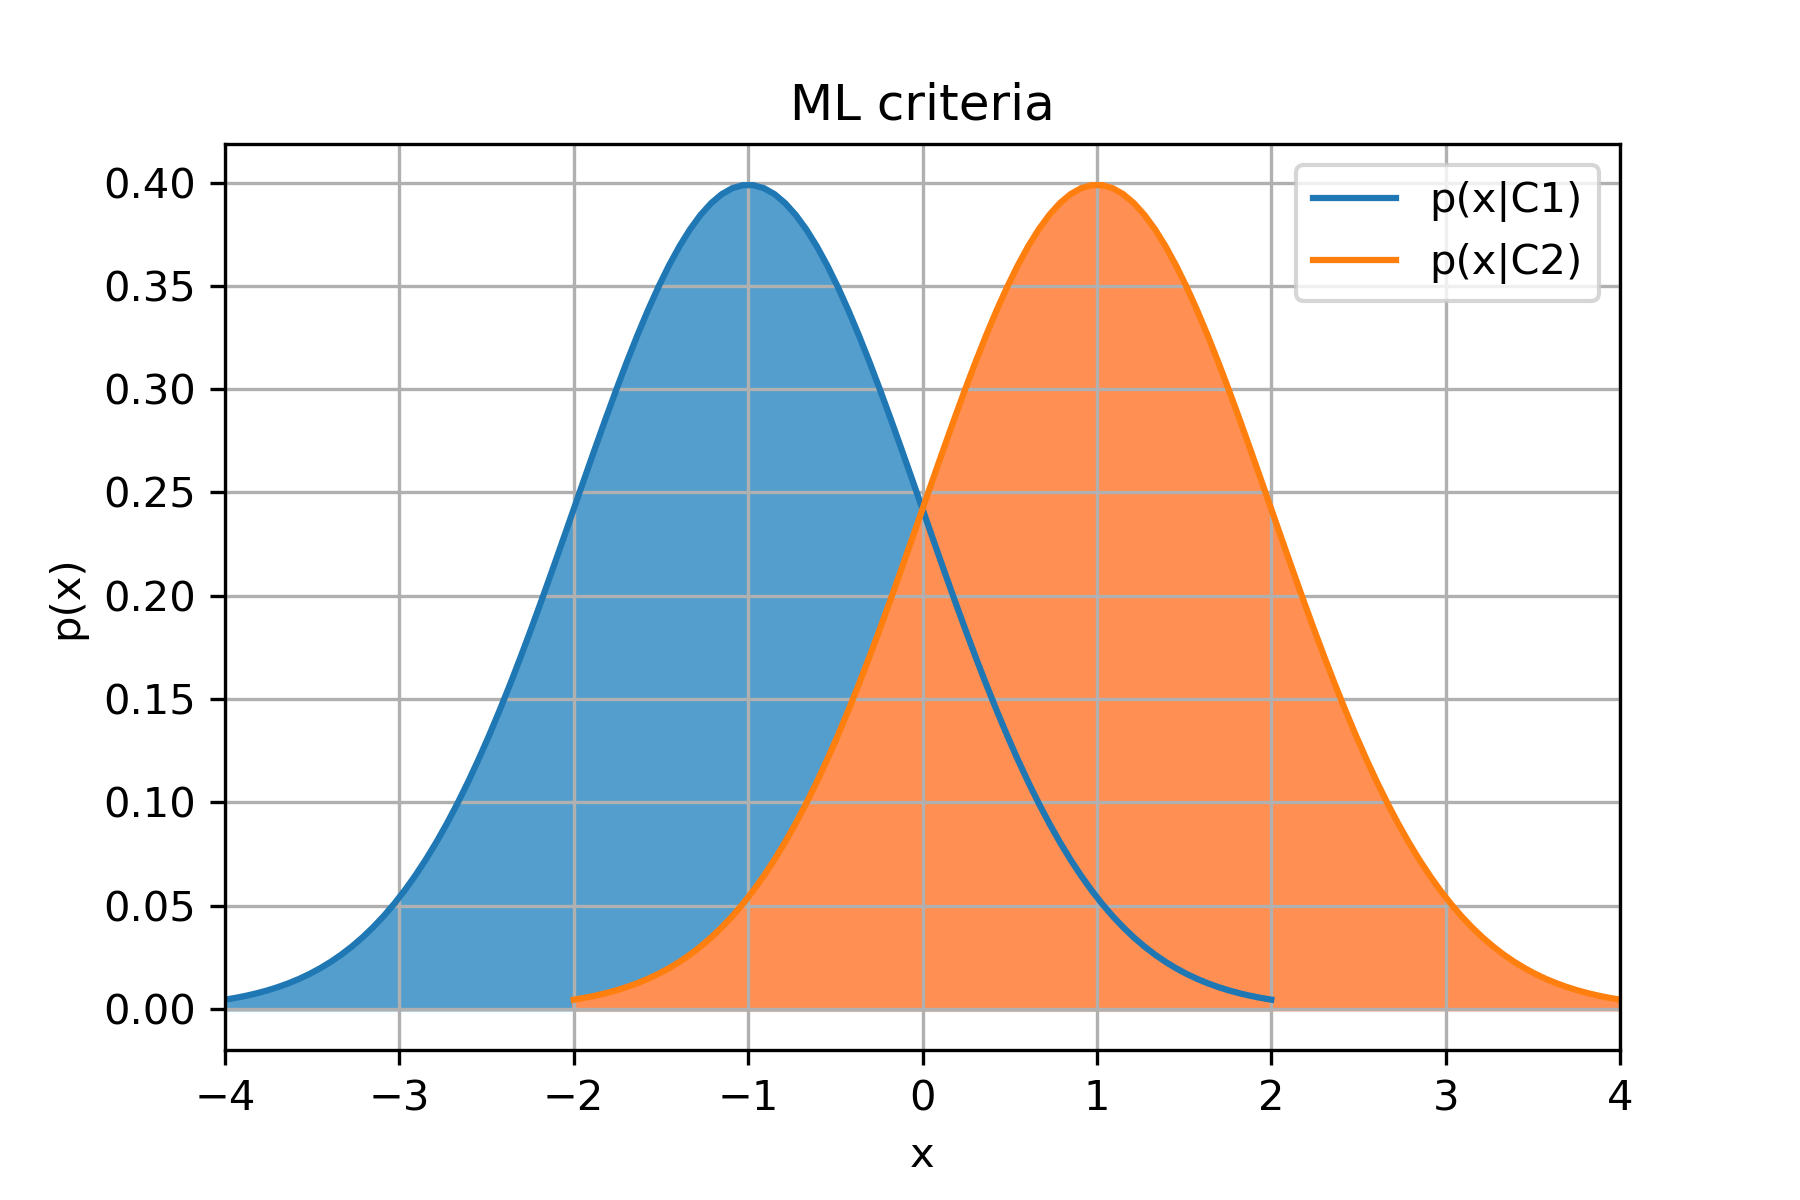
\includegraphics[width=12cm]{ML}
    \caption{Visualization of C1 and C2 distributions under the ML criteria}
    \label{fig:ML}
\end{figure}

As we can see in the \ref{fig:ML}

%==============================
\subsubsection{b) Calcule P(X = 0|Y = 0).}
%==============================

$$ p(C_1) = 0.7 $$
$$ p(C_2) = 0.3 $$

%Através do critério MAP, temos que x pertence a classe C_1 se p(C_1|x) > p(C_2|x):

$$ p(C_1|x) > p(C_2|x) $$

Aplicando a regra de Bayes, temos:

$$ \frac{p(x|C_1)\cdot p(C_1)}{p(x)} > \frac{p(x|C_2)\cdot p(C_2)}{p(x)} $$

$$ \frac{1}{\sqrt{2\pi\sigma_1^2}}exp\left(-\frac{(x-\mu_1)^2}{2 \sigma_1^2}\right)\cdot p(C_1) > \frac{1}{\sqrt{2\pi\sigma_2^2}}exp\left(-\frac{(x-\mu_2)^2}{2 \sigma_2^2}\right) \cdot p(C_2) $$

$$ \frac{1}{\sqrt{2\pi\cdot1^2}}exp\left(-\frac{(x-(-1))^2}{2\cdot1^2}\right) (0.7) > \frac{1}{\sqrt{2\pi\cdot1^2}}exp\left(-\frac{(x-1)^2}{2\cdot1^2}\right) (0.3) $$

$$ exp\left(-\frac{(x+1)^2}{2}\right) (0.7) > exp\left(-\frac{(x-1)^2}{2}\right) (0.3) $$

Tirando o ln de ambos os lados:

$$ -\frac{(x+1)^2}{2} + \ln(0.7) > -\frac{(x-1)^2}{2} + \ln(0.3) $$

$$ -x^2-2x-1 + 2\ln(0.7) > -x^2+2x-1 + 2\ln(0.3)    $$
$$ -2x + 2\ln(0.7) > 2x + 2\ln(0.3)                 $$
$$ -x + \ln(0.7) > x + \ln(0.3)                     $$
$$ 2x  < \ln(0.7) - \ln(0.3)                        $$
$$ x  < \frac{\ln(0.7) - \ln(0.3)}{2}               $$
$$ \boxed{x  < 0.4236}                              $$

\begin{figure}[h]
    \centering
    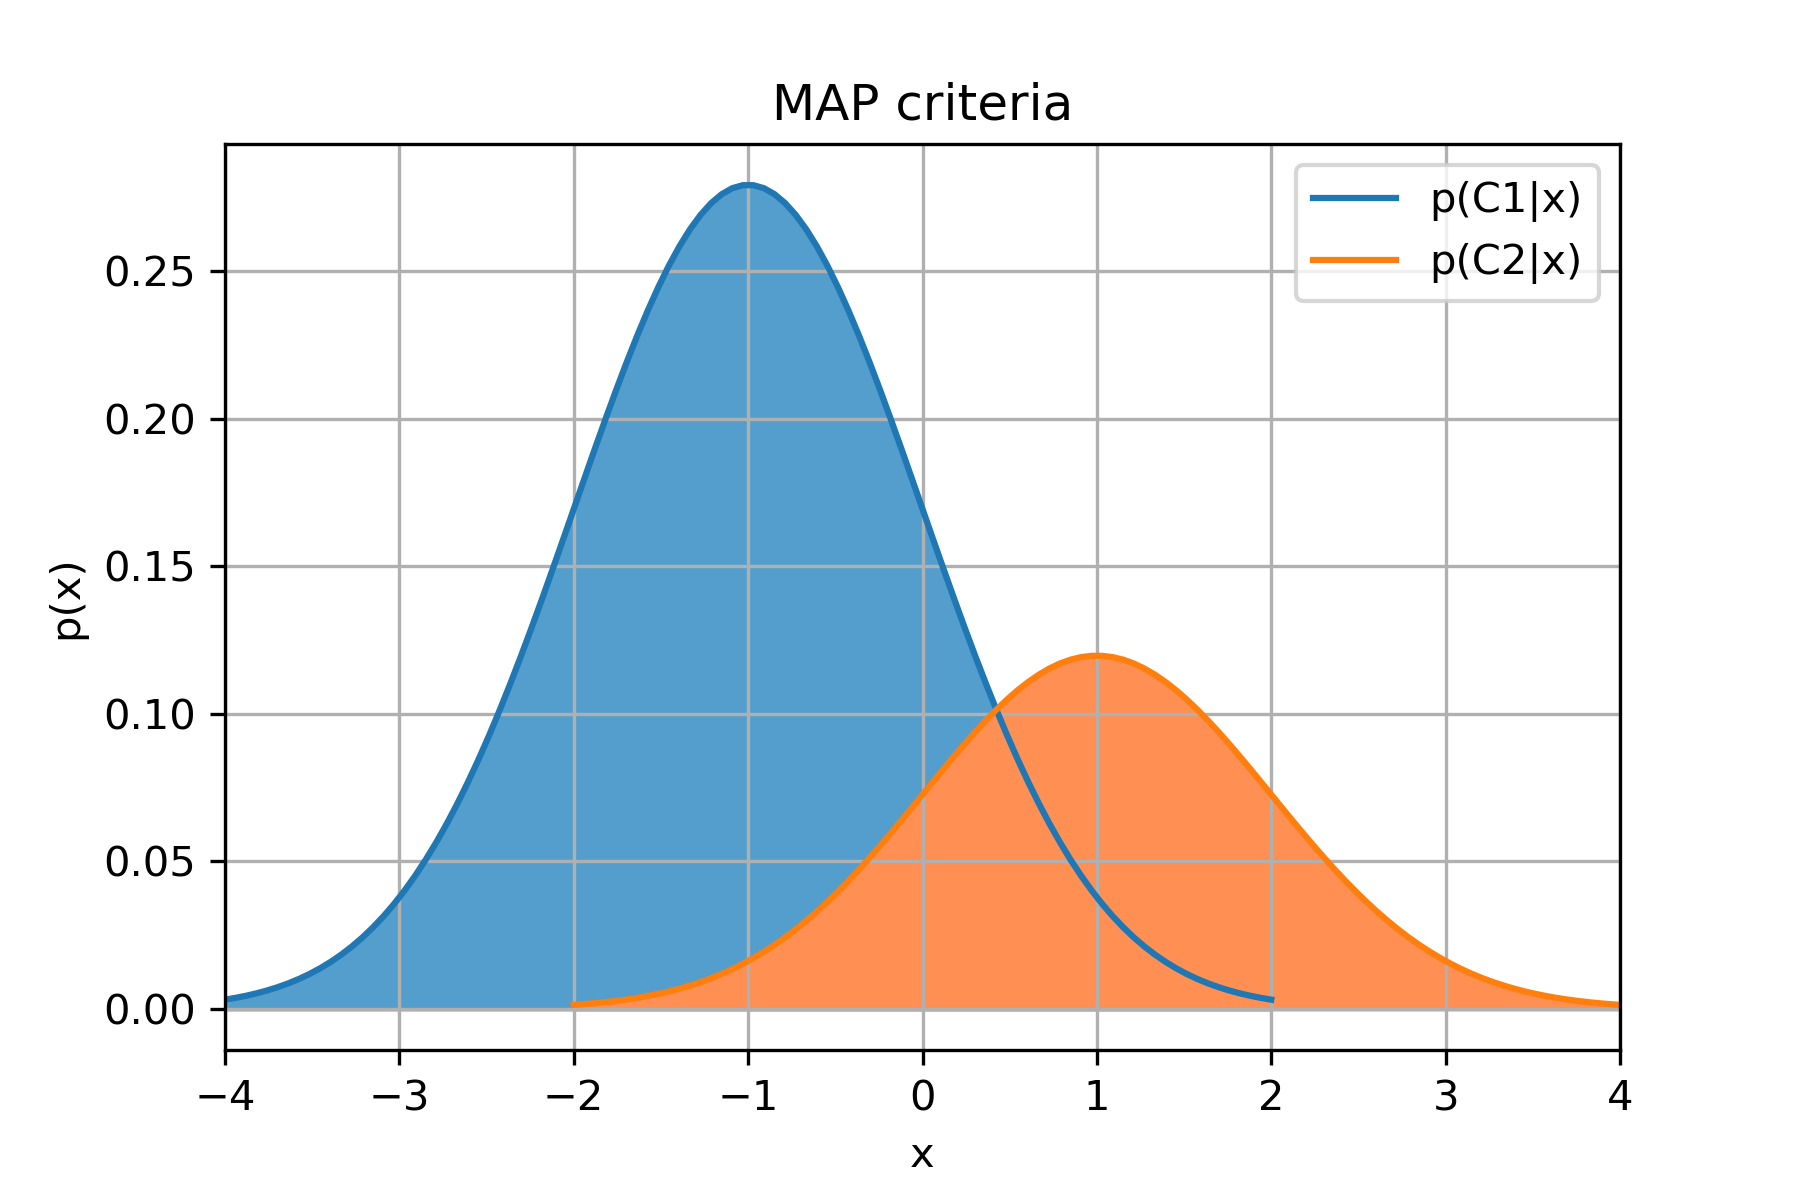
\includegraphics[width=12cm]{MAP}
    \caption{Vizualization of C1 and C2 distributions under the MAP criteria}
    \label{fig:MAP}
\end{figure}

As we can see in the \ref{fig:MAP}

%=================================================
\section{Computational Activites}
%=================================================

\paragraph{
All code presented and all figures showed here can be found at the following GitHub repository:\\
\url{https://github.com/ito-rafael/IA006C-MachineLearning}\\
In this repository, one can found the following files:\\
}

\begin{itemize}
    \item Jupyter Notebook
    \begin{itemize}
        \item \href{https://github.com/ito-rafael/IA006C-MachineLearning/blob/master/efc1/theoretical-ex.ipynb}{theoretical-ex.ipynb}
        \item \href{https://github.com/ito-rafael/IA006C-MachineLearning/blob/master/efc1/pre-ex1.ipynb}{pre-ex1.ipynb}
        \item \href{https://github.com/ito-rafael/IA006C-MachineLearning/blob/master/efc1/pre-ex2.ipynb}{pre-ex2.ipynb}
        \item \href{https://github.com/ito-rafael/IA006C-MachineLearning/blob/master/efc1/ex1.ipynb}{ex1.ipynb}
        \item \href{https://github.com/ito-rafael/IA006C-MachineLearning/blob/master/efc1/ex2.ipynb}{ex2.ipynb}
    \end{itemize}
    \item Python code
    \begin{itemize}
        \item \href{https://github.com/ito-rafael/IA006C-MachineLearning/blob/master/efc1/ex1.py}{ex1.py}
        \item \href{https://github.com/ito-rafael/IA006C-MachineLearning/blob/master/efc1/ex2.py}{ex2.py}
    \end{itemize}
    \item \LaTeX
    \begin{itemize}
        \item \href{}{efc1.tex}
    \end{itemize}
\end{itemize}

\paragraph{The notebook "theoretical-ex.ipynb" is used to generate the figures \ref{fig:ML} and \ref{fig:MAP}. The notebook "pre-ex1" is used only for data visualization. It shows how the dataset is split in order to use the k-fold cross-validation method. The notebook "pre-ex2" has a similar used than the previous one. It is used to visualize the data, but besides the raw data, it also plots the dataset linearly transformed before and after the application of the hyperbolic tangent function. The two last notebooks, "ex1" and "ex2" actually implements all the functions to train the models and that answers the exercises 1 and 2.}
\paragraph{The Python codes presented contain the same code of the notebooks. Finally, the \LaTeX file is the source code to generate this pdf.}

%=======================================
\subsection{Exercise 1}
%=======================================

\paragraph{The first thing we did before starting this exercise was to plot all the data, as can be seen in figure \ref{fig:pre-ex1-0}.}

\begin{figure}[ht]
    \centering
    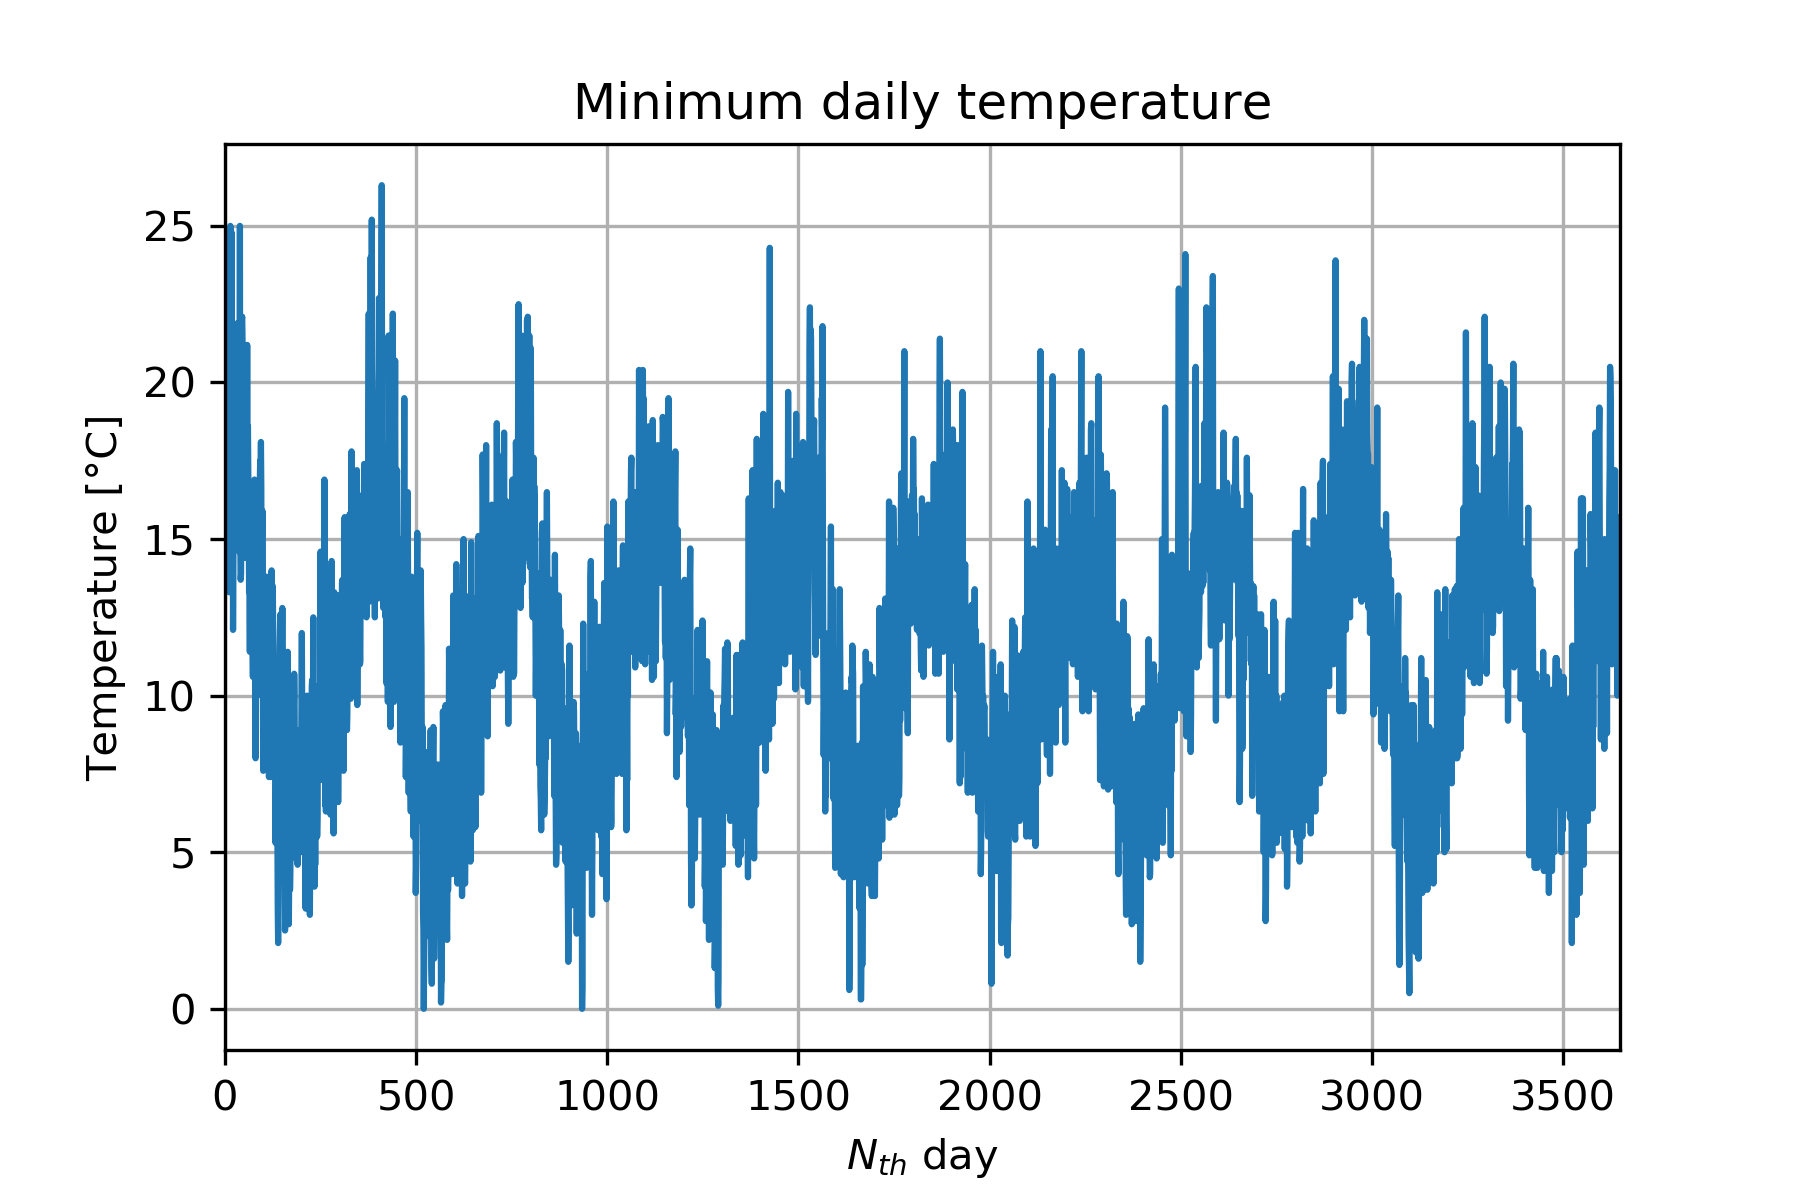
\includegraphics[width=12cm]{figure_0_all_data}
    \caption{All data}
    \label{fig:pre-ex1-0}
\end{figure}

\paragraph{The next step was to decide the number of folds used in the k-fold cross-validation method. Since we are treating a time series forecasting problem, it was decided to split the dataset equally to the number of the years of the dataset excluding the data used to test the model: nine. When creating the folds, a method like the one that is showed in figure \ref{fig:pre-ex1-folds} was used.}

\begin{figure}[ht]
    \centering
    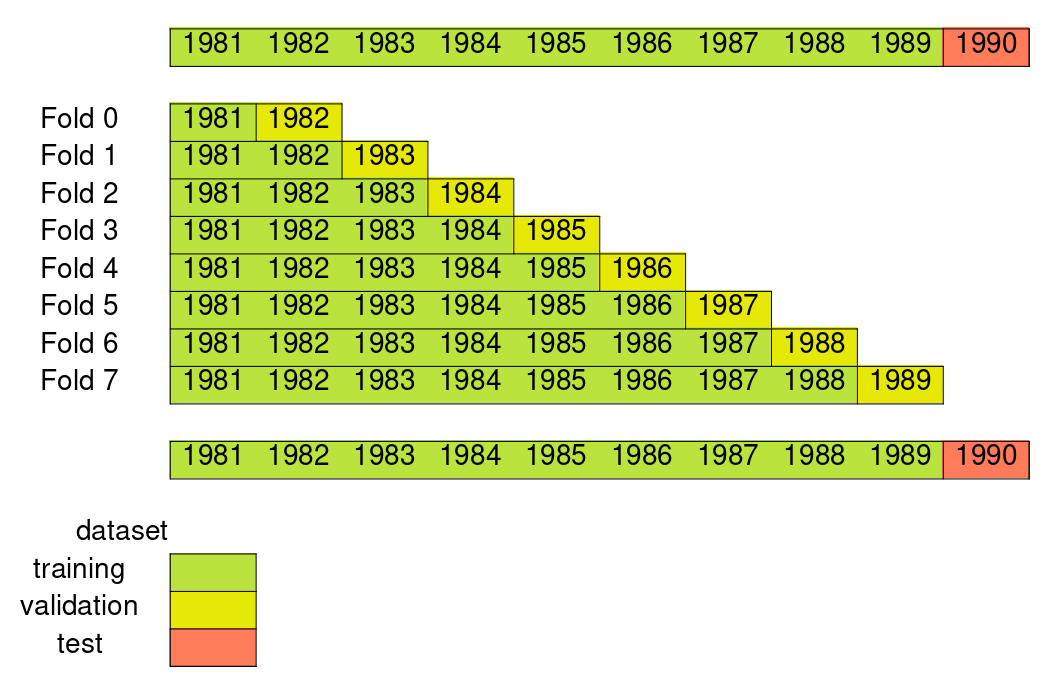
\includegraphics[width=12cm]{figure_0_kfold}
    \caption{Folds used to cross-validate the model}
    \label{fig:pre-ex1-folds}
\end{figure}

\paragraph{In this method, only past data is used to predict forward-looking data. The first fold is formed by only the first year of the dataset, the year 1981, while the year used at the validation step is the next year, 1982. The second fold uses all the data of the previous fold (train plus validation) as the data to be trained, and the next year, 1983, as the validation data. Doing this for all the folds we get the configuration showed in figure \ref{fig:pre-ex1-kfolds}.}

\begin{figure}
    \centering
    % all data
    \begin{subfigure}{0.32\textwidth}
        \centering
        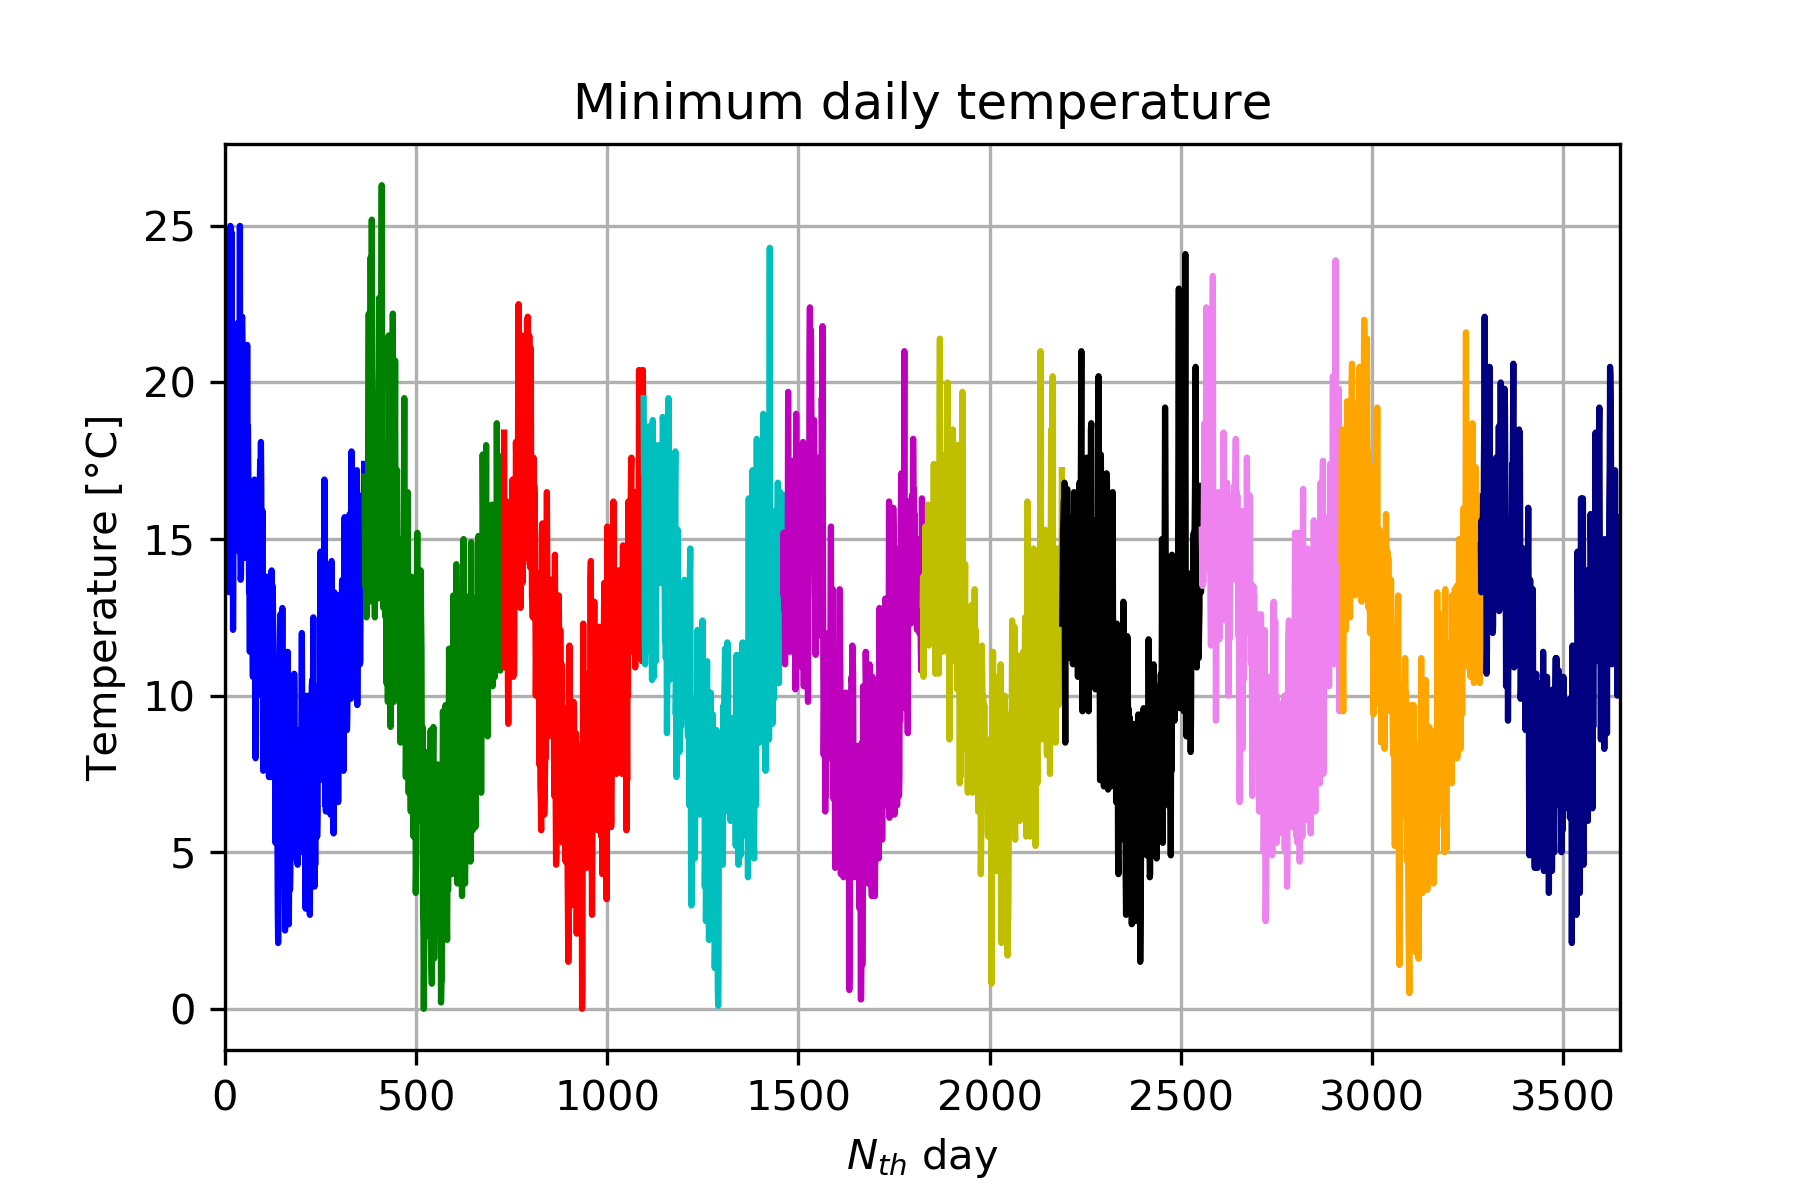
\includegraphics[width=3.85cm]{figure_1_data_split}
        \caption{Dataset split}
        \label{fig:sub1}
    \end{subfigure}
    \hfill
    % fold 1
    \begin{subfigure}{0.32\textwidth}
        \centering
        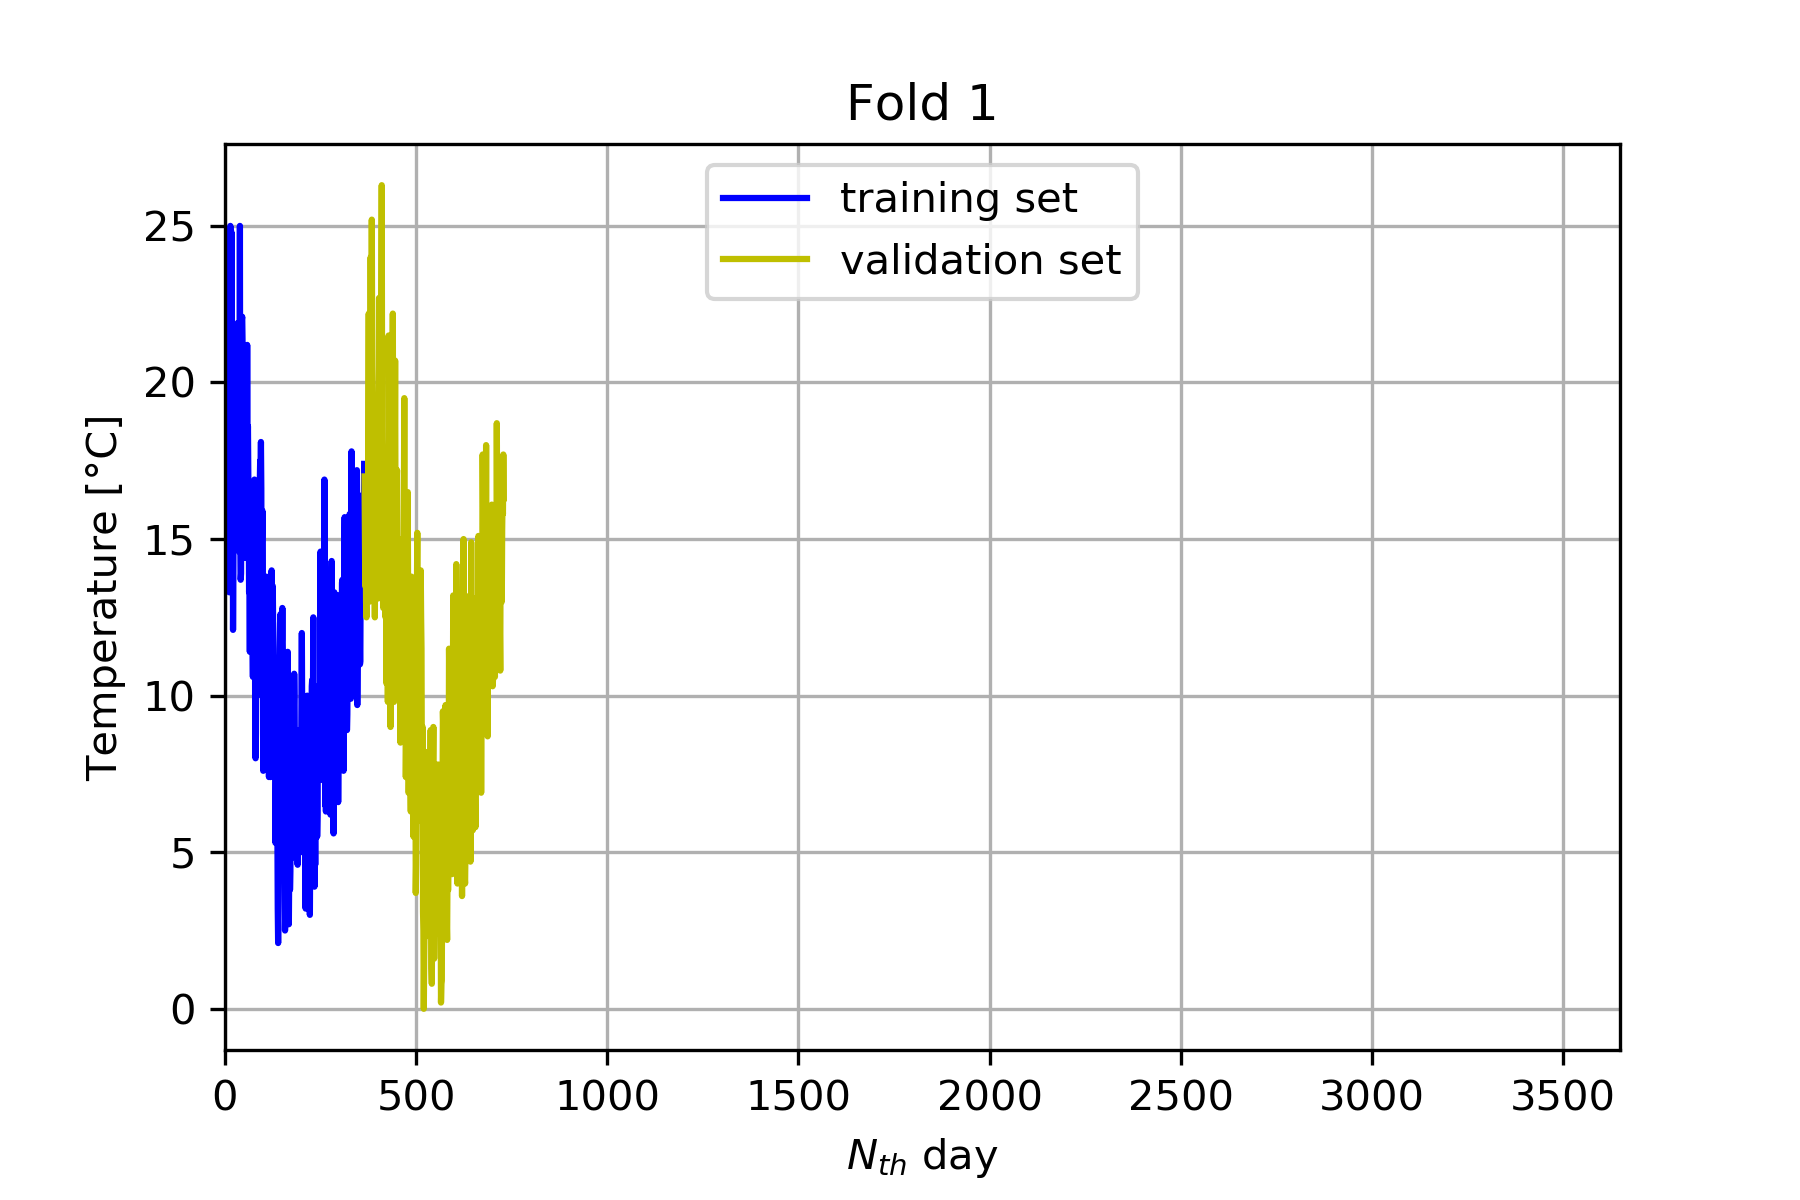
\includegraphics[width=3.85cm]{figure_2_fold_1}
        \caption{Fold 1}
        \label{fig:sub2}
    \end{subfigure}
    \hfill
    % fold 2
    \begin{subfigure}{0.32\textwidth}
        \centering
        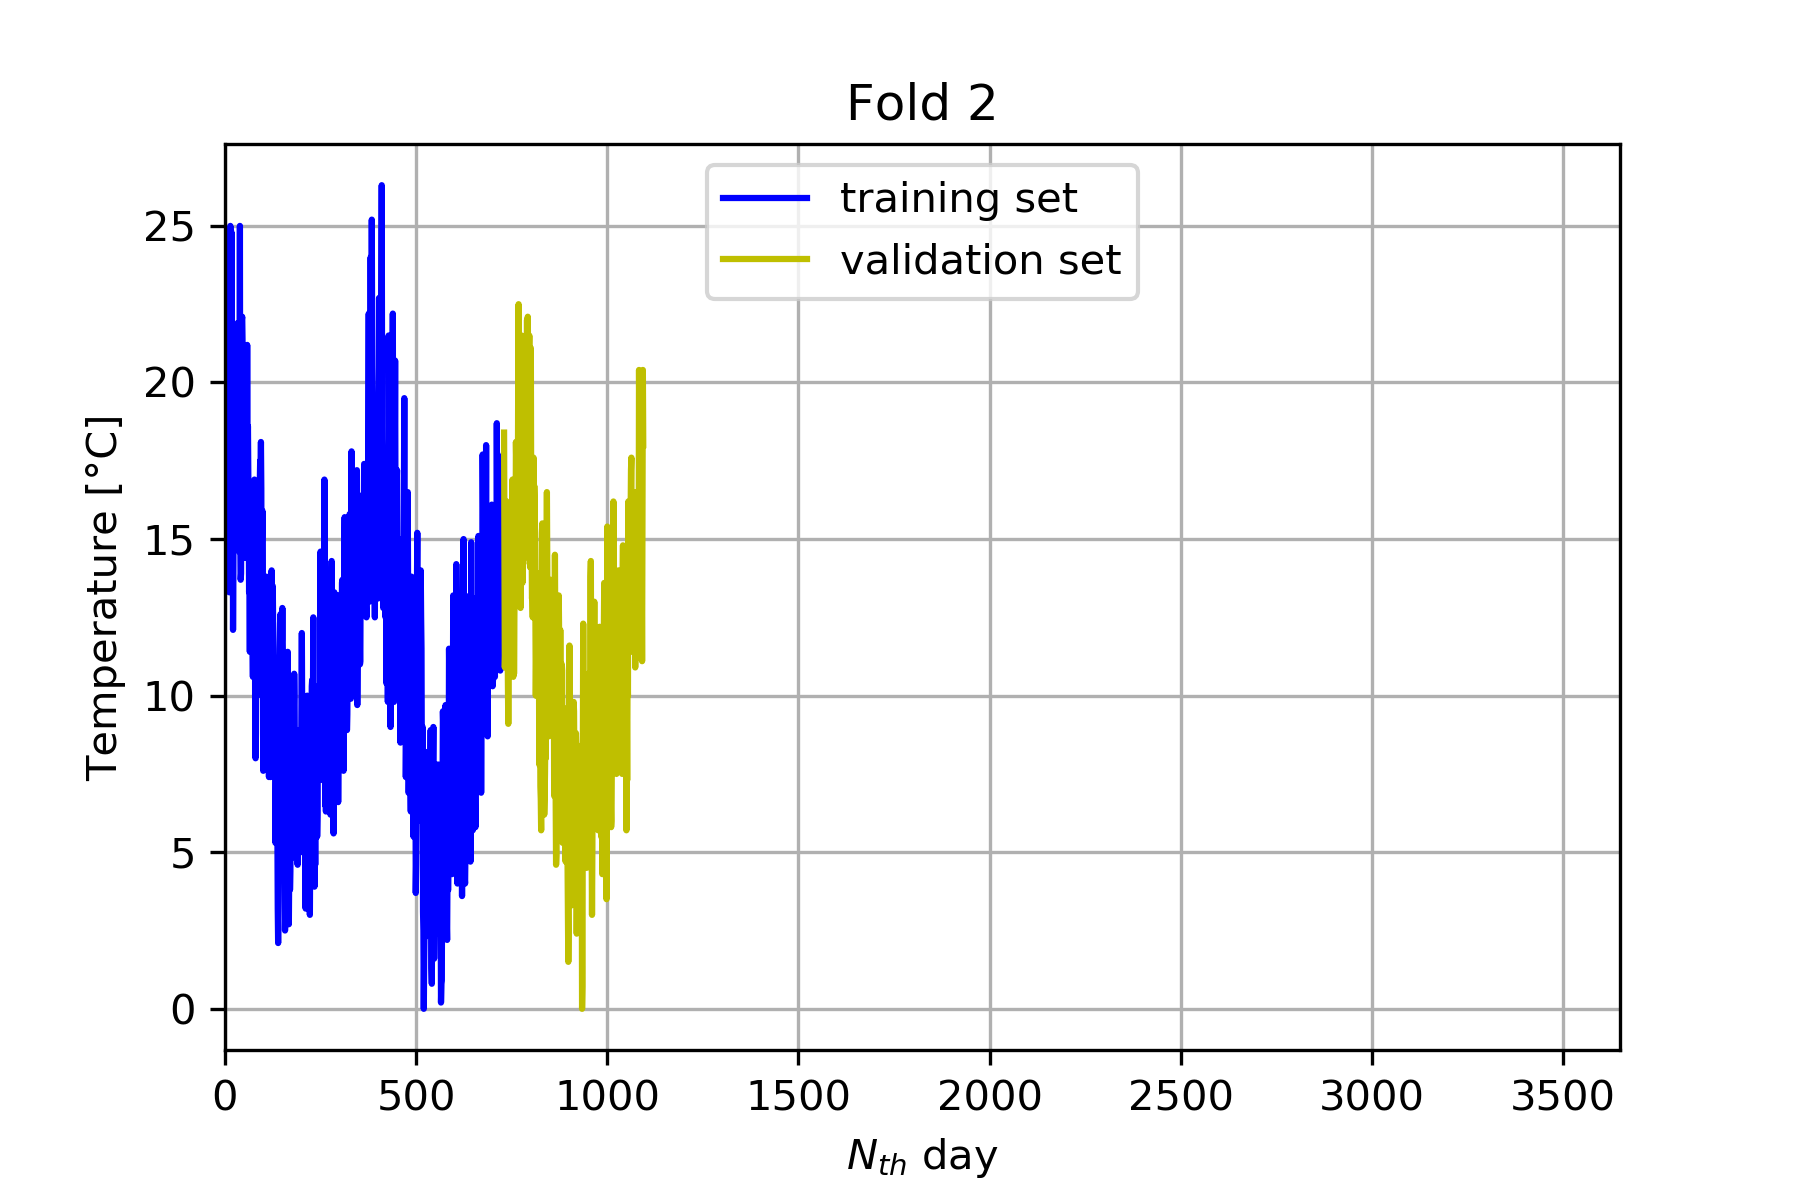
\includegraphics[width=3.85cm]{figure_3_fold_2}
        \caption{Fold 2}
        \label{fig:sub3}
    \end{subfigure}%
    \\
    % fold 3
    \begin{subfigure}{0.32\textwidth}
        \centering
        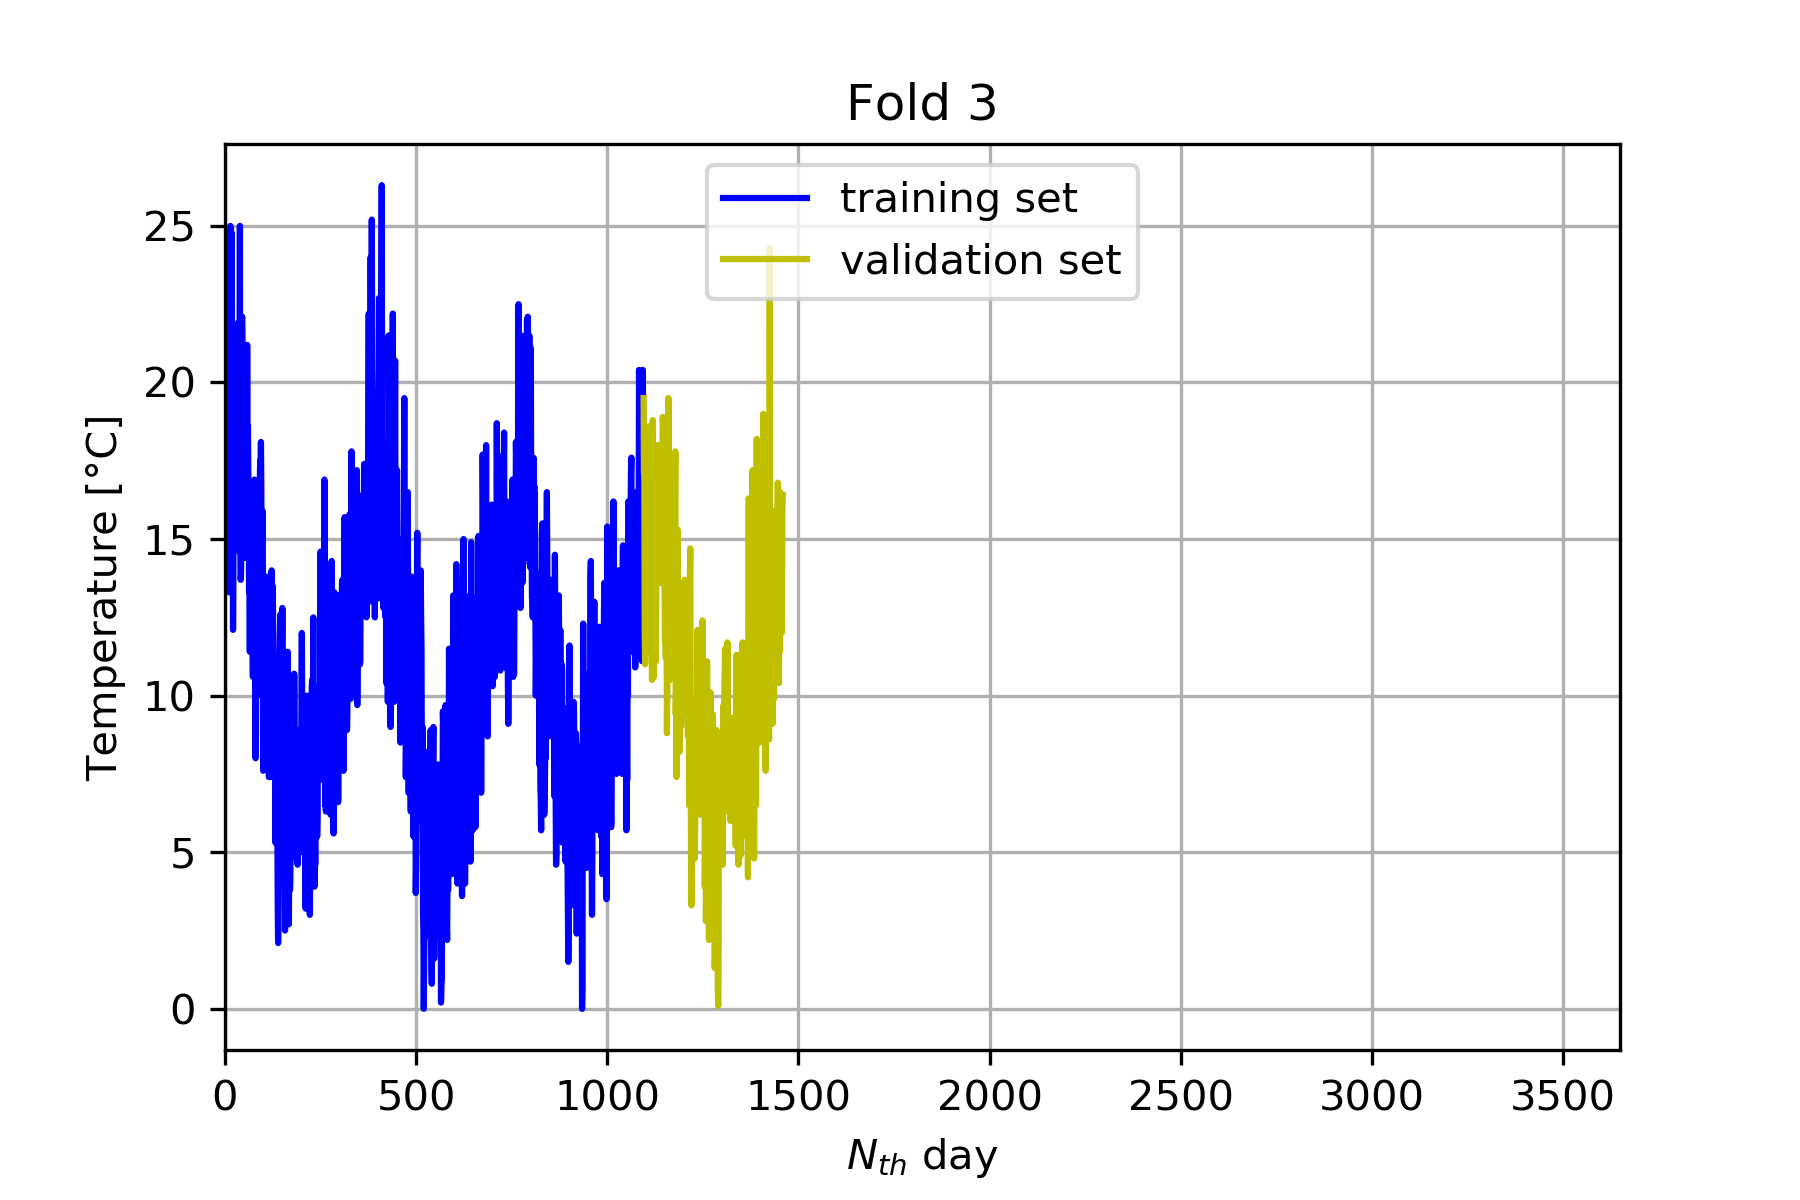
\includegraphics[width=3.85cm]{figure_4_fold_3}
        \caption{Fold 3}
        \label{fig:sub4}
    \end{subfigure}\hfill
    % fold 4
    \begin{subfigure}{0.32\textwidth}
        \centering
        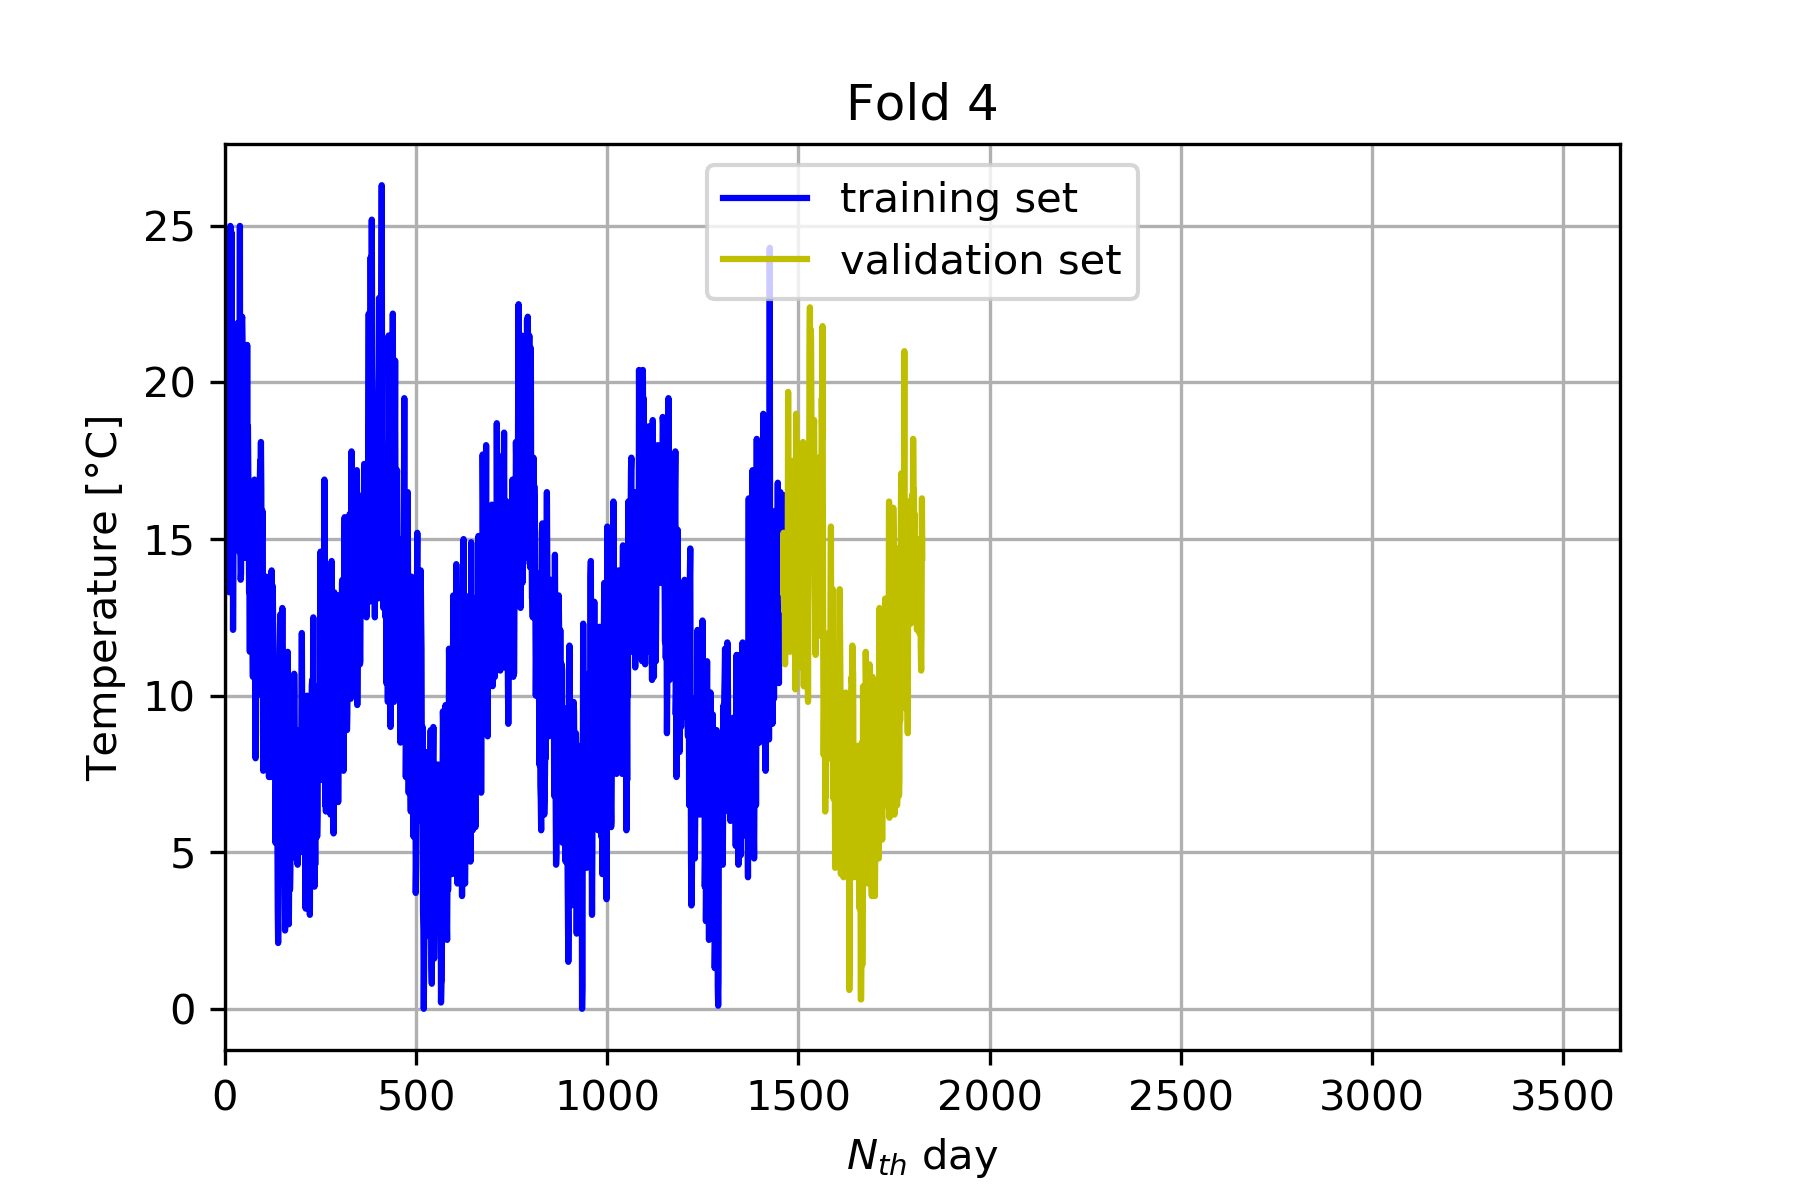
\includegraphics[width=3.85cm]{figure_5_fold_4}
        \caption{Fold 4}
        \label{fig:sub5}
    \end{subfigure}\hfill
    % fold 5
    \begin{subfigure}{0.32\textwidth}
        \centering
        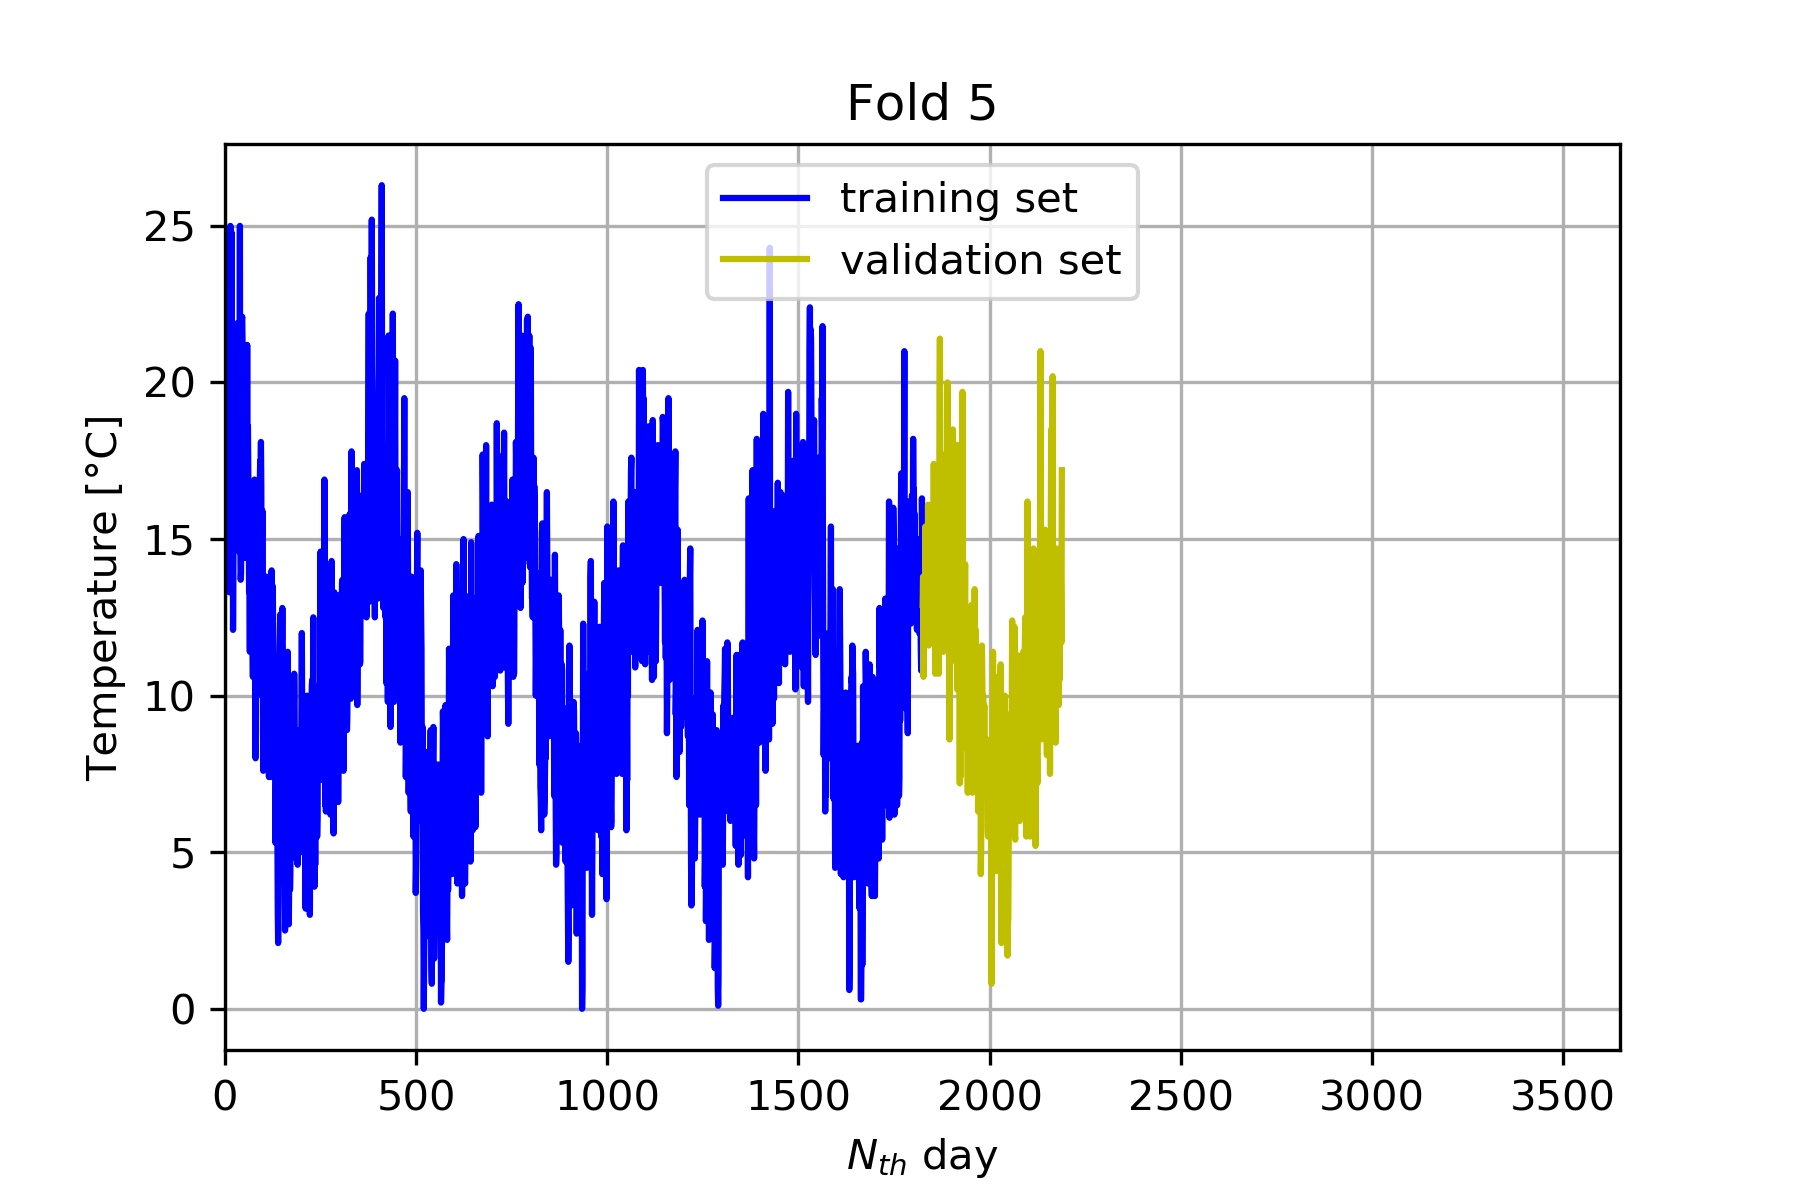
\includegraphics[width=3.85cm]{figure_6_fold_5}
        \caption{Fold 5}
        \label{fig:sub6}
    \end{subfigure}
    \\
    % fold 6
    \begin{subfigure}{0.32\textwidth}
        \centering
        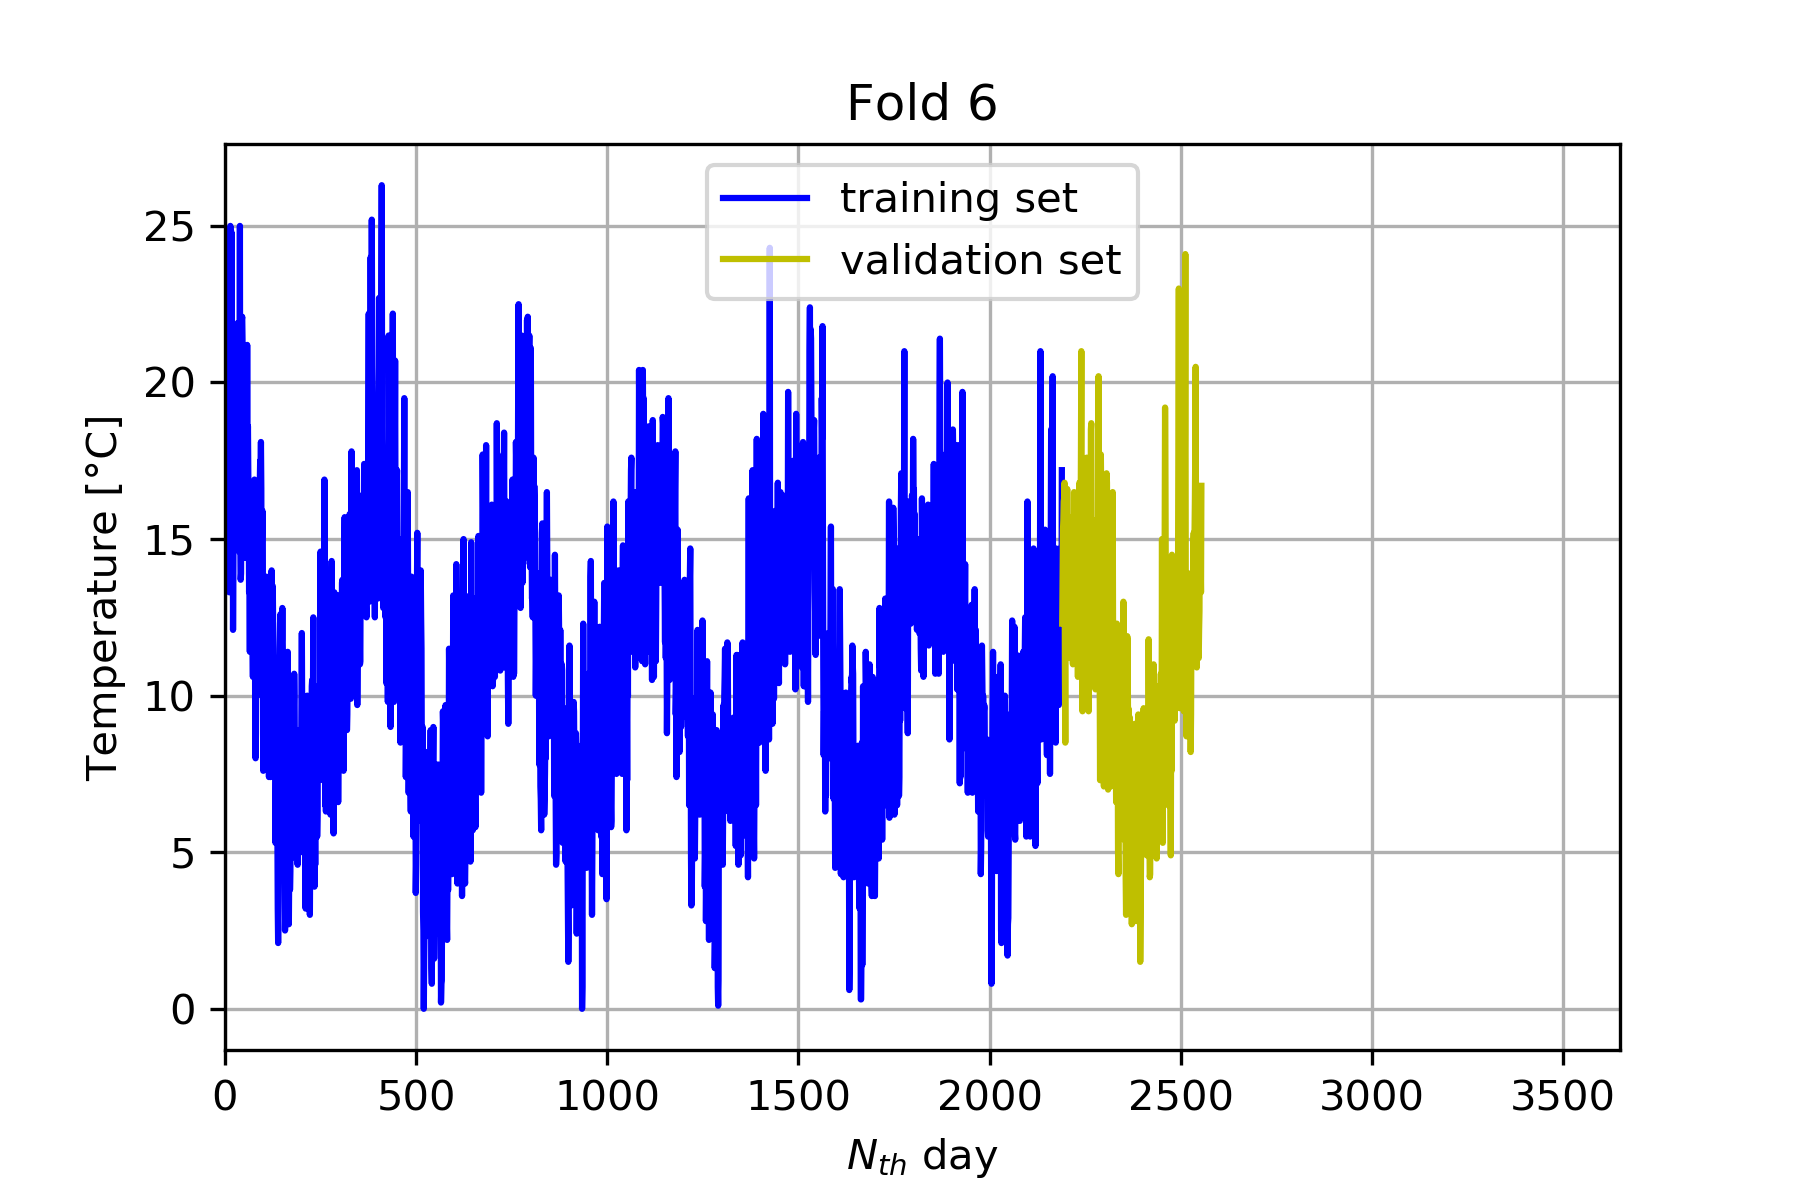
\includegraphics[width=3.85cm]{figure_7_fold_6}
        \caption{Fold 6}
        \label{fig:sub7}
    \end{subfigure}\hfill
    % fold 7
    \begin{subfigure}{0.32\textwidth}
        \centering
        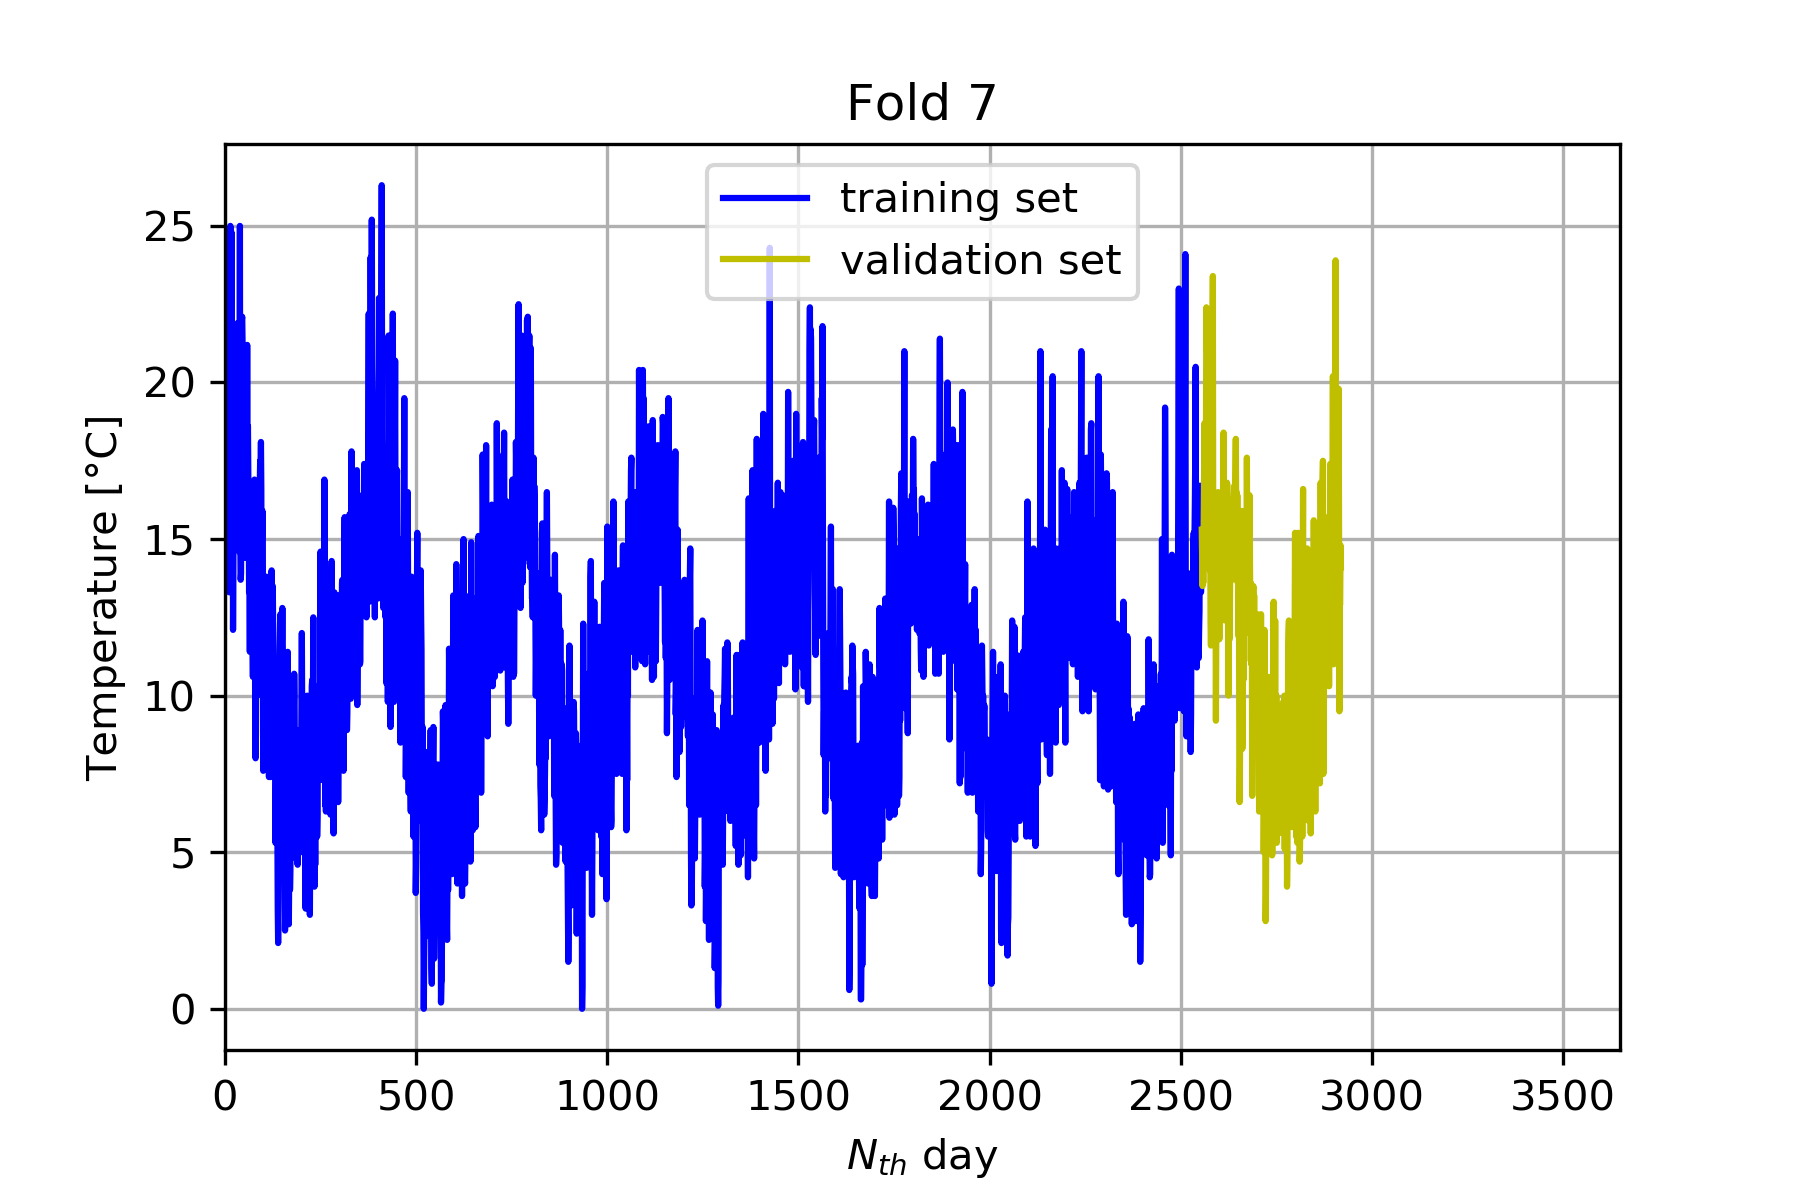
\includegraphics[width=3.85cm]{figure_8_fold_7}
        \caption{Fold 7}
        \label{fig:sub8}
    \end{subfigure}\hfill
    % fold 8
    \begin{subfigure}{0.32\textwidth}
        \centering
        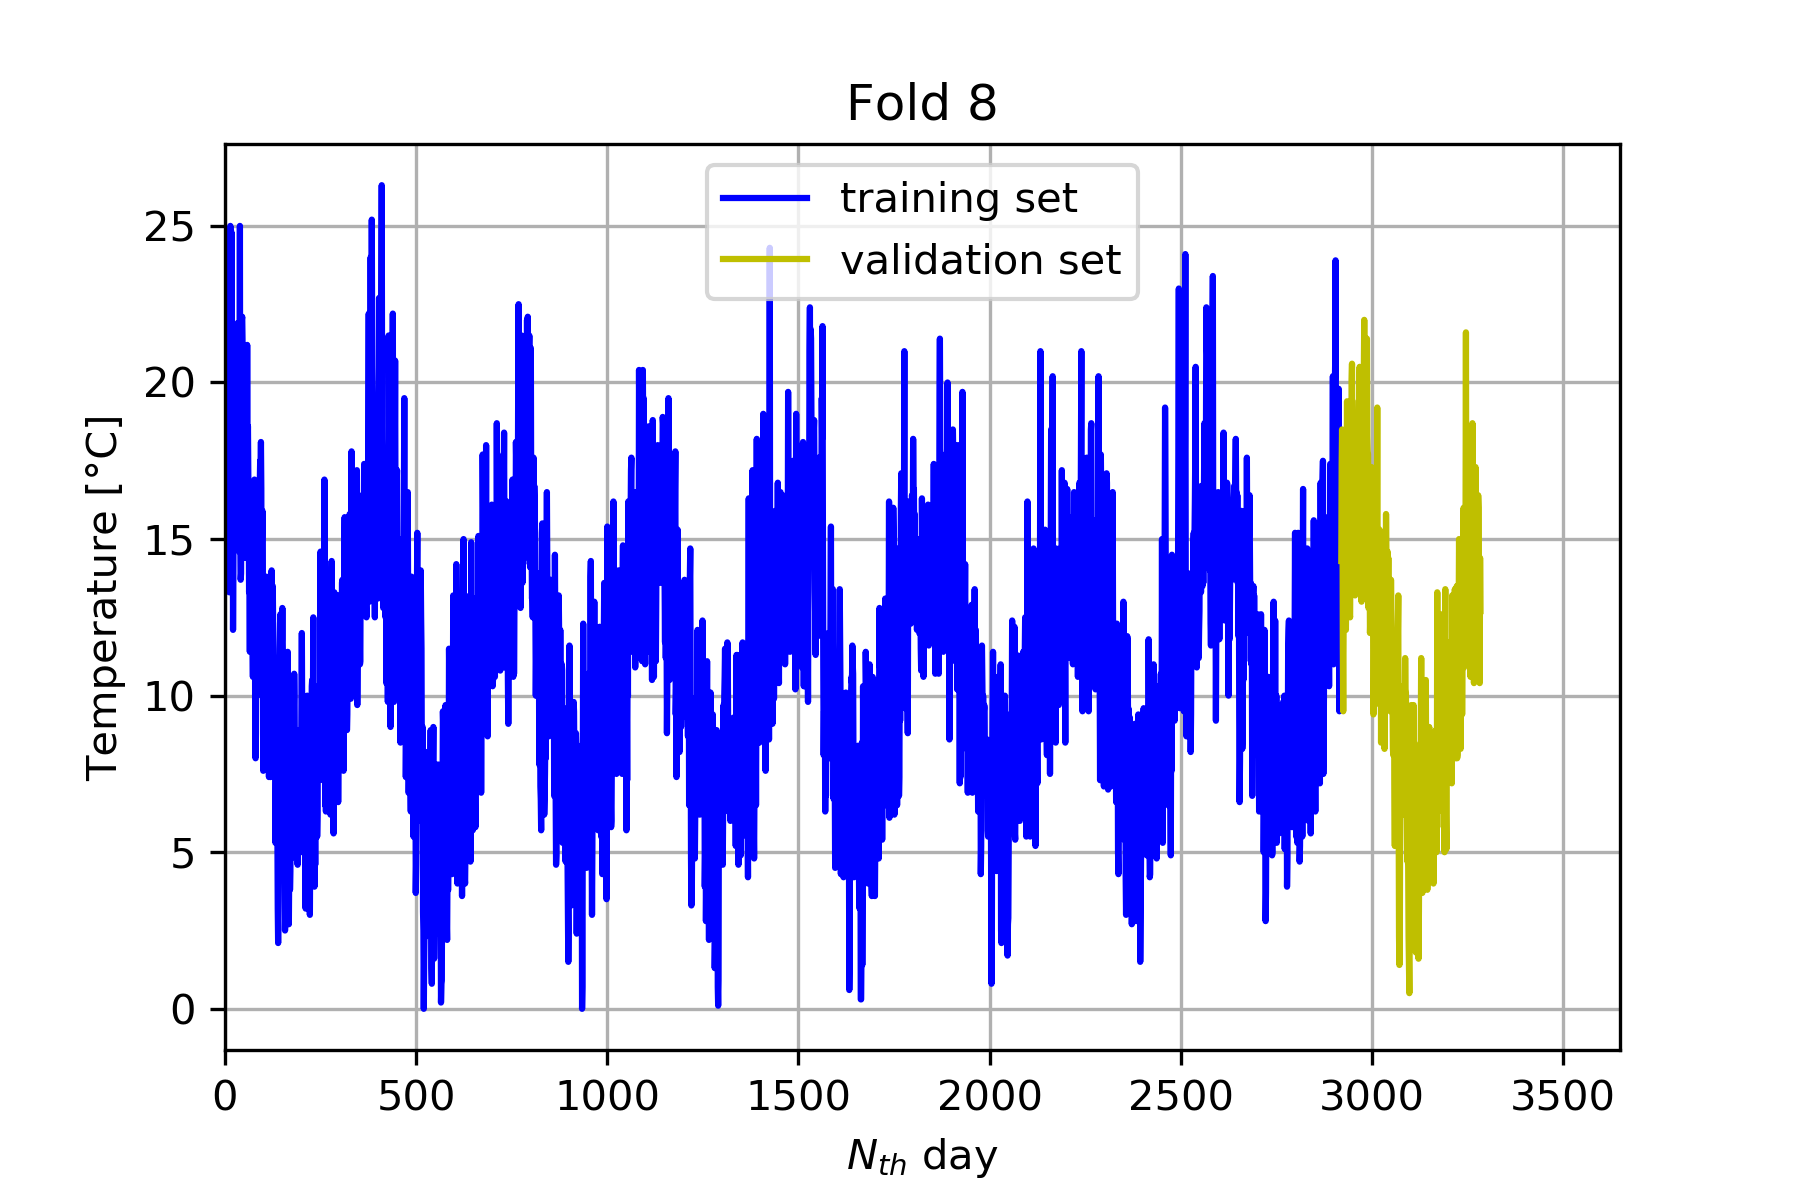
\includegraphics[width=3.85cm]{figure_9_fold_8}
        \caption{Fold 8}
        \label{fig:sub9}
    \end{subfigure}
    % caption and label
    \caption{Folds used in cross-validation}
    \label{fig:pre-ex1-kfold}
\end{figure}

\paragraph{The goal of using this method of cross-validation is to find the best value for the hyperparameter K, the number of previous days used as input for the model.\\After choosing the hyperparater, we no more use the folds division. Instead, all data before used for training and validation is now used only for training. This can be considered as the last training of the model and the one which will return the weights desired in this problem of linear regression. This can be seen in figure \ref{fig:pre-ex1-10}.}

\begin{figure}[ht]
    \centering
    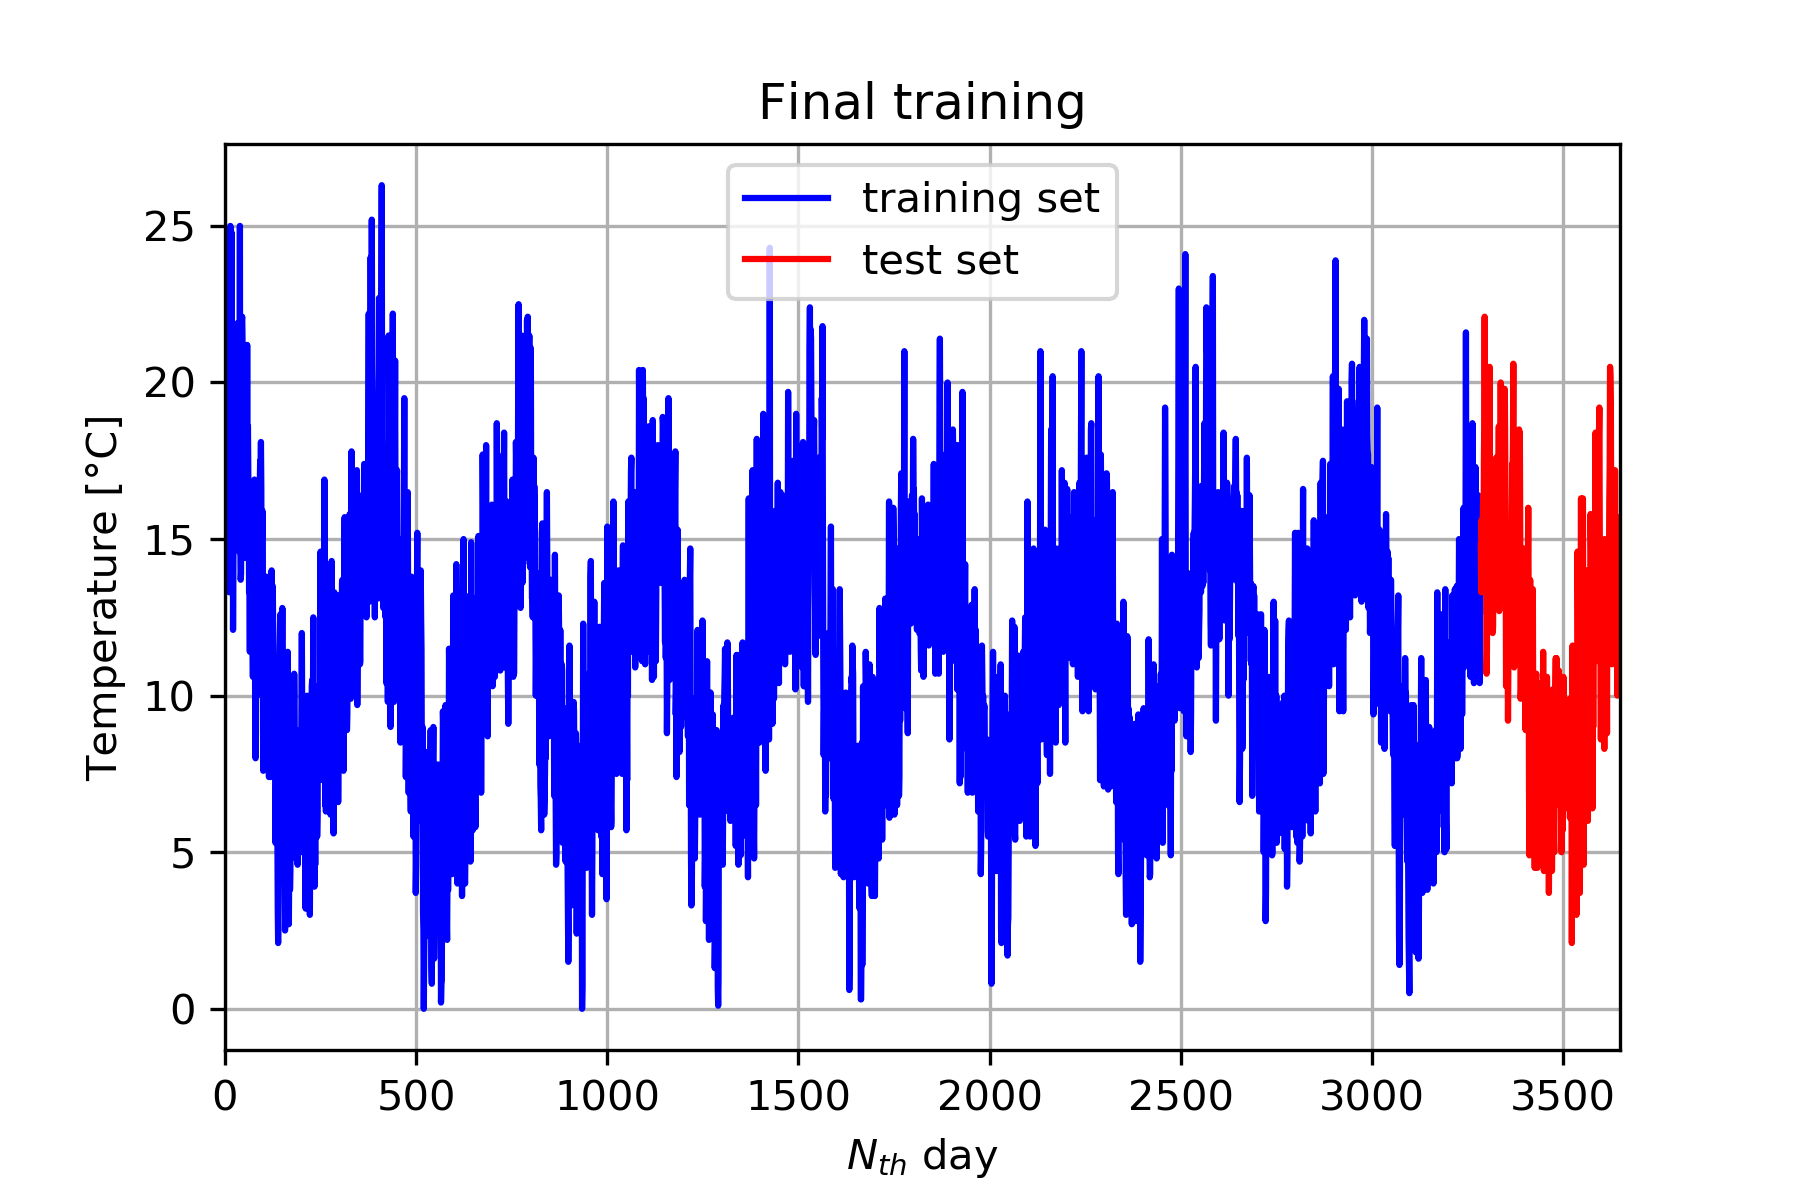
\includegraphics[width=12cm]{figure_10_final_training}
    \caption{}
    \label{fig:pre-ex1-10}
\end{figure}

%==============================
\subsubsection{a) Progression of RMSE measured in validation set in function of hyperparameter K (from 1 to 31):}
%==============================

\paragraph{The model was trained for values of the hyperparameter K from 1 to 31 days. The progression of the root mean squared error (RMSE) measured in the validation set can be seen in figure \ref{fig:ex1-1}.}

\begin{figure}[ht]
    \centering
    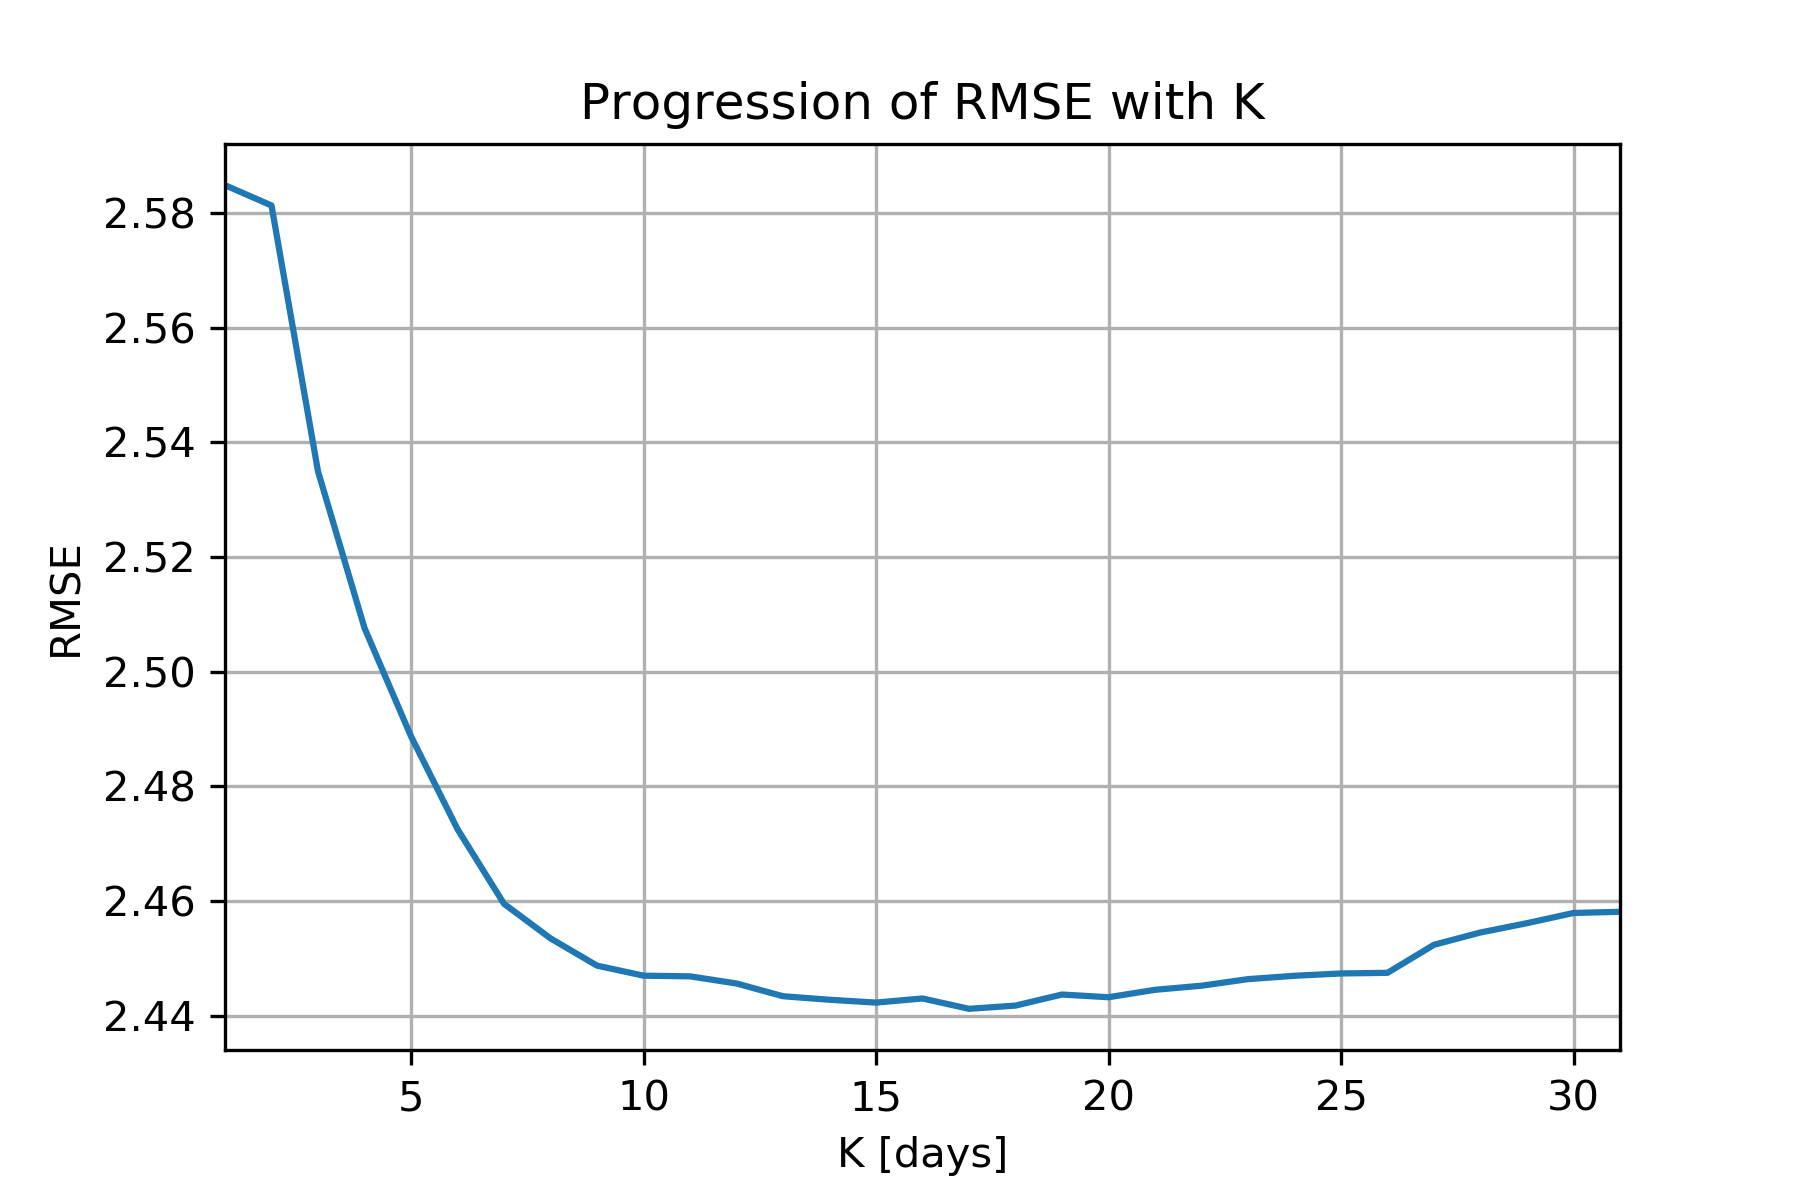
\includegraphics[width=12cm]{figure_1_rmse_with_k}
    \caption{}
    \label{fig:ex1-1}
\end{figure}

\paragraph{asd}

\begin{figure}[ht]
    \centering
    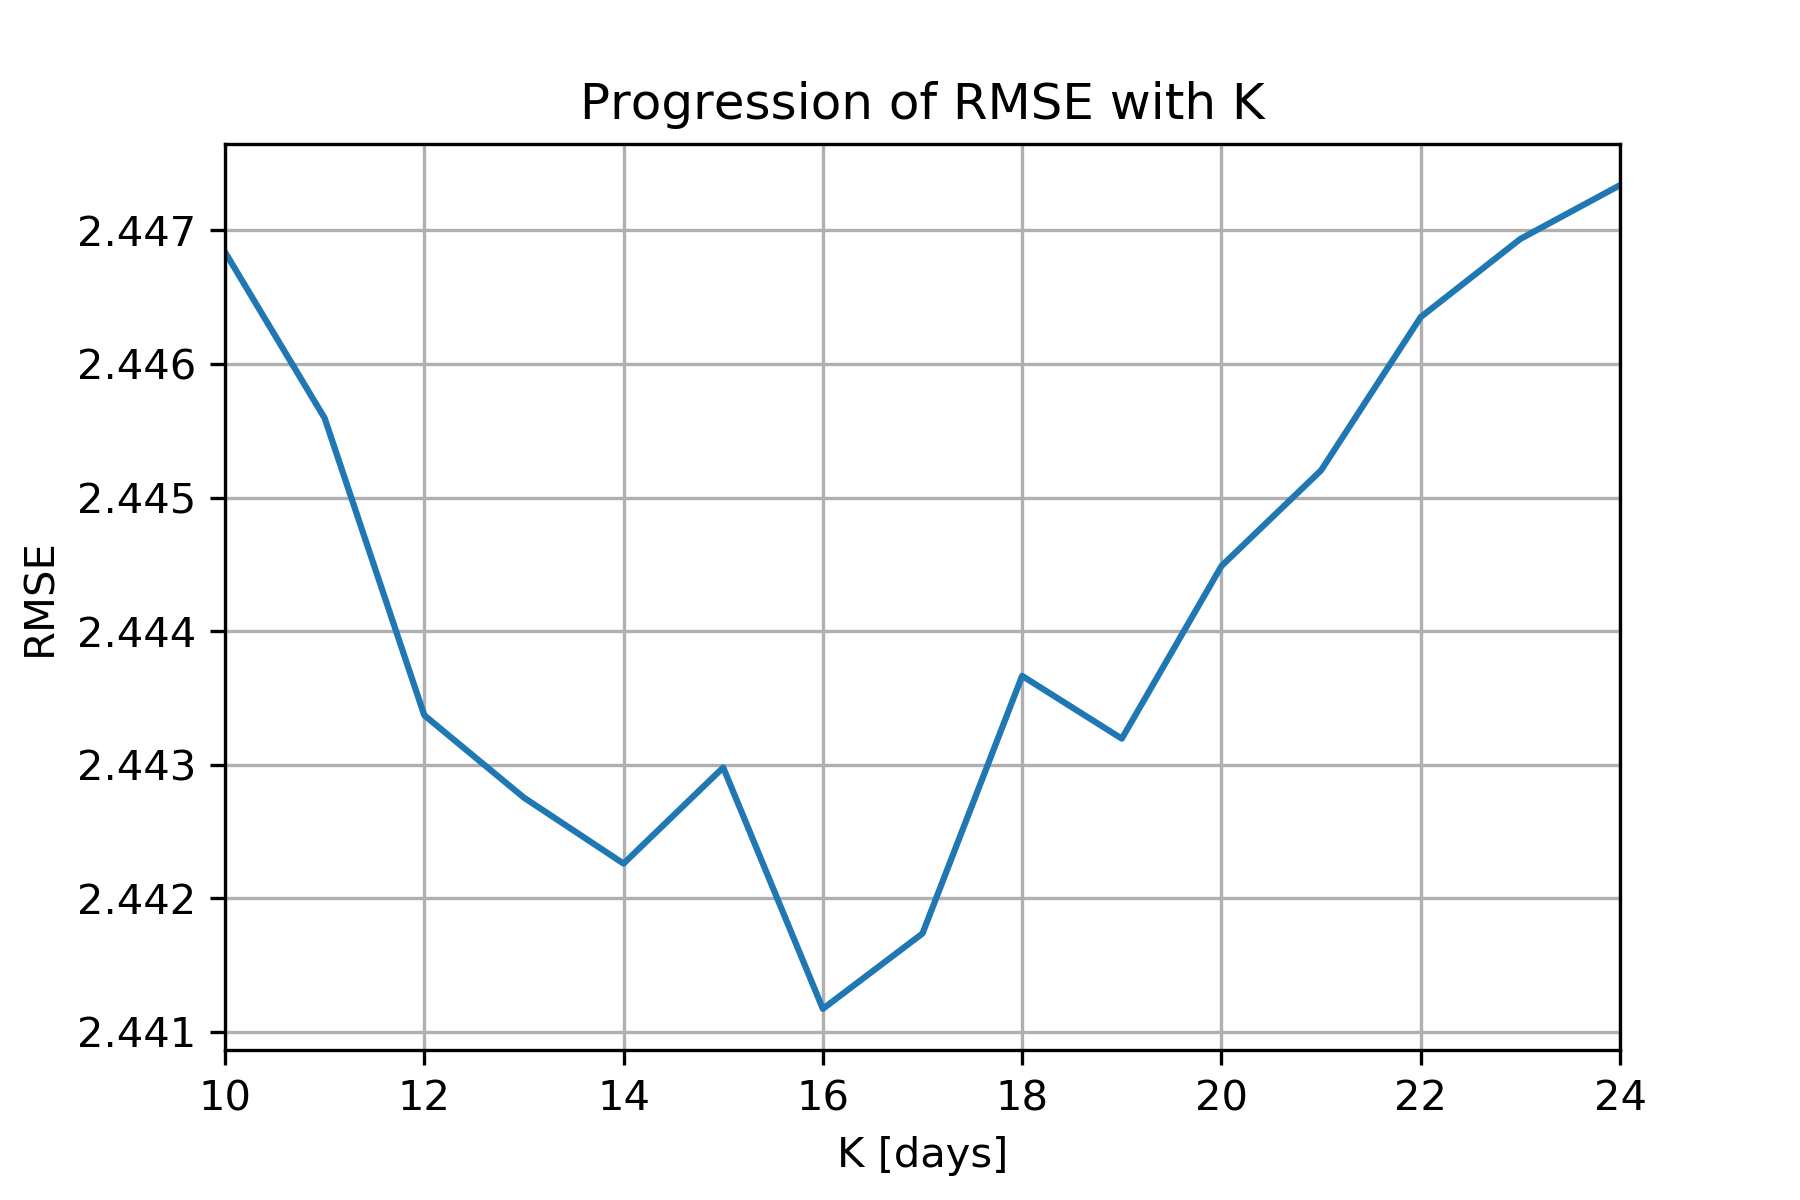
\includegraphics[width=12cm]{figure_2_rmse_with_k_zoom}
    \caption{}
    \label{fig:ex1-2}
\end{figure}

%==============================
\subsubsection{b) Plot of predicted and real temperatures of test set}
%==============================

\begin{figure}[ht]
    \centering
    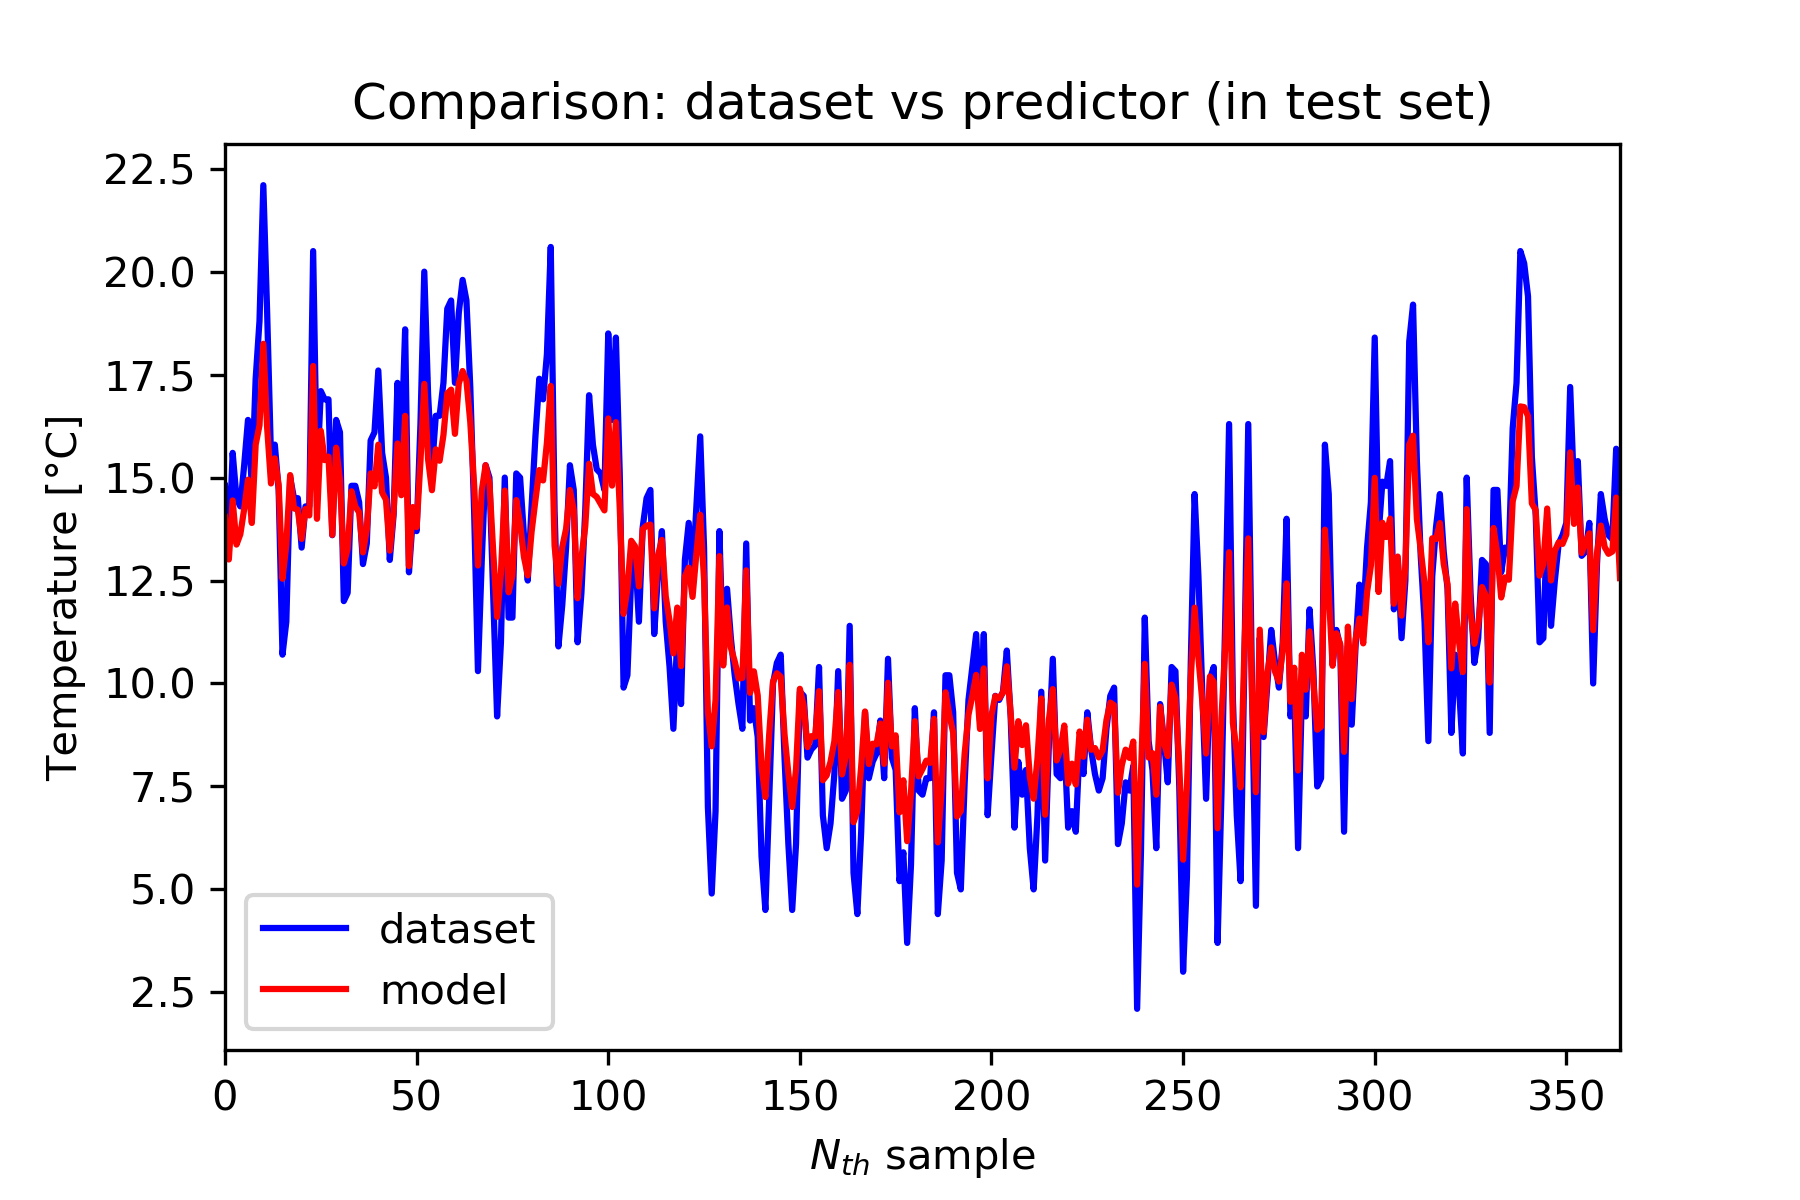
\includegraphics[width=12cm]{figure_3_predictor}
    \caption{}
    \label{fig:ex1-3}
\end{figure}

%=======================================
\subsection{Exercise 2}
%=======================================

\begin{figure}[ht]
    \centering
    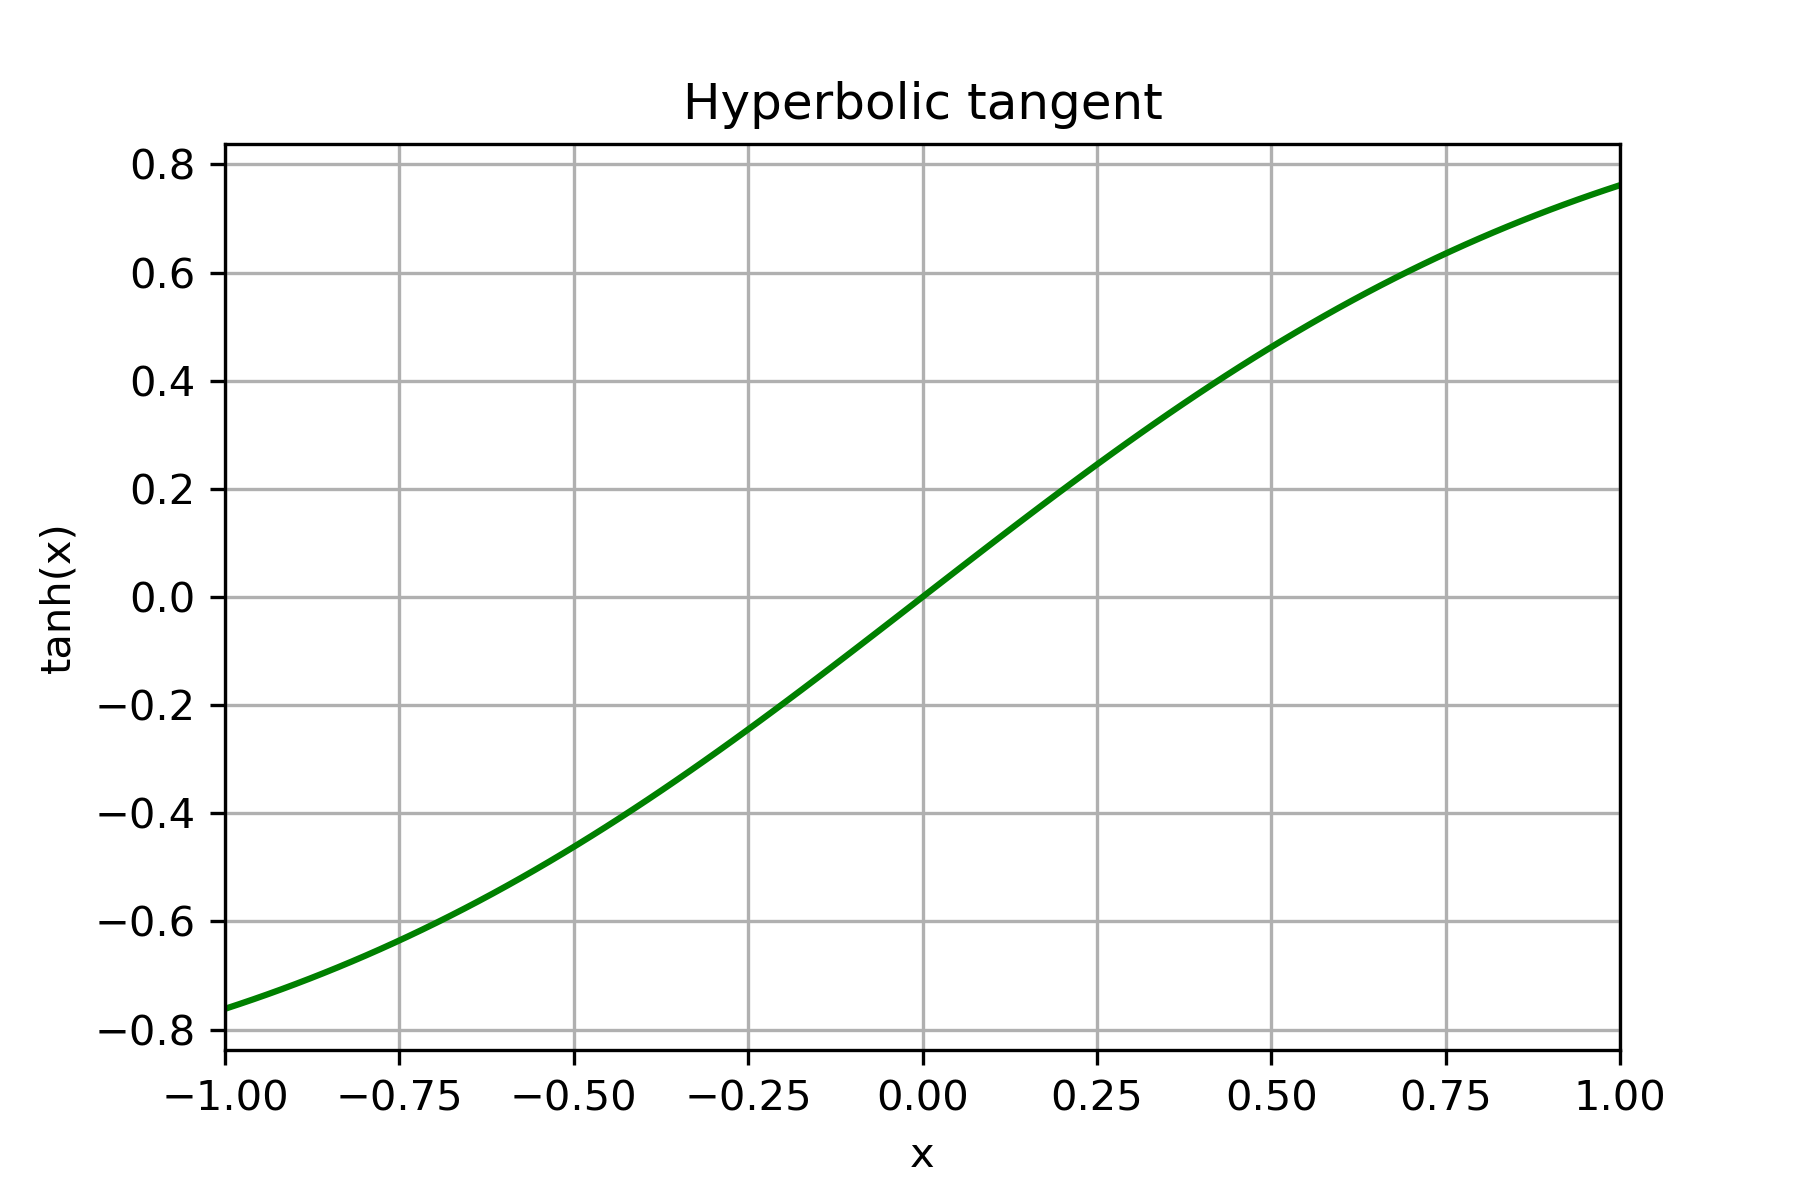
\includegraphics[width=12cm]{figure_1_hyperbolic_tangent}
    \caption{}
    \label{fig:pre-ex2-1}
\end{figure}

\begin{figure}[ht]
    \centering
    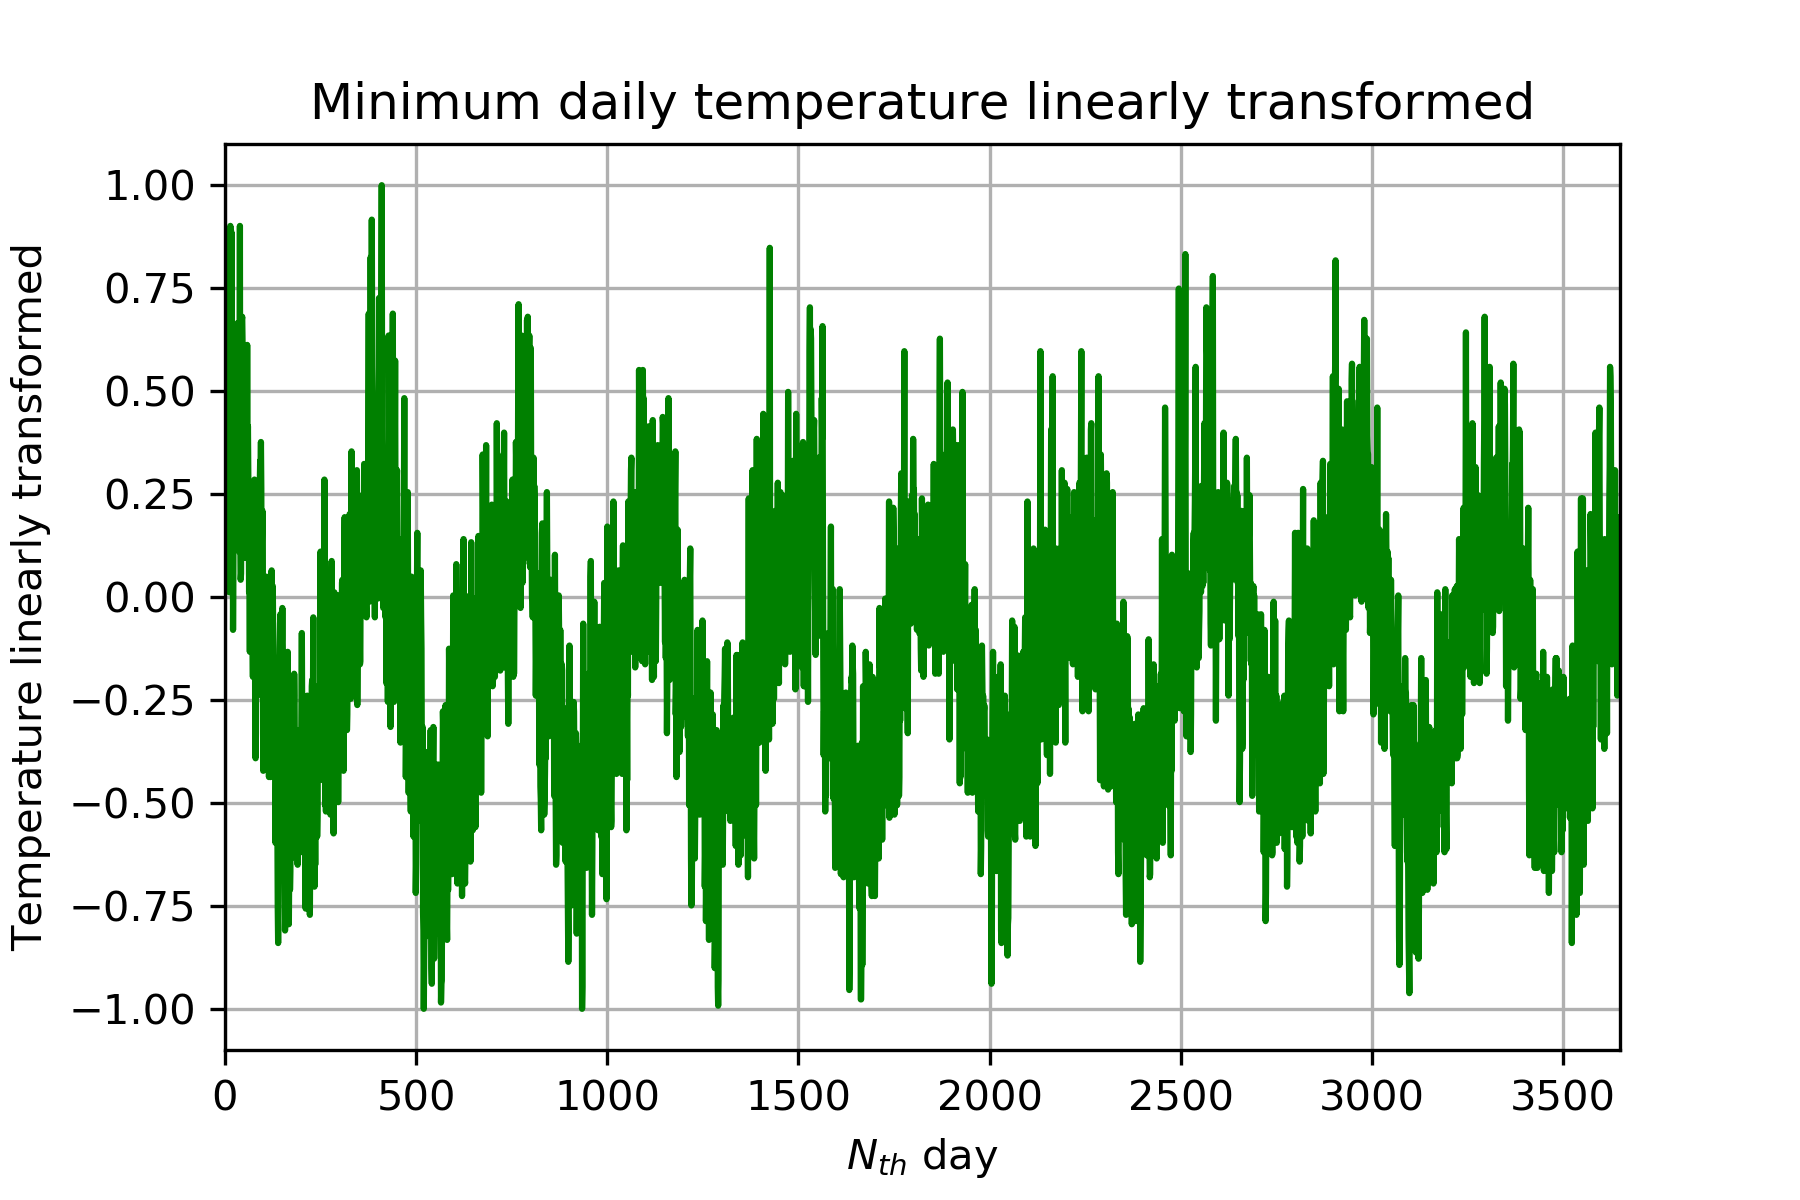
\includegraphics[width=12cm]{figure_2_linear_transformation}
    \caption{}
    \label{fig:pre-ex2-2}
\end{figure}

\begin{figure}[ht]
    \centering
    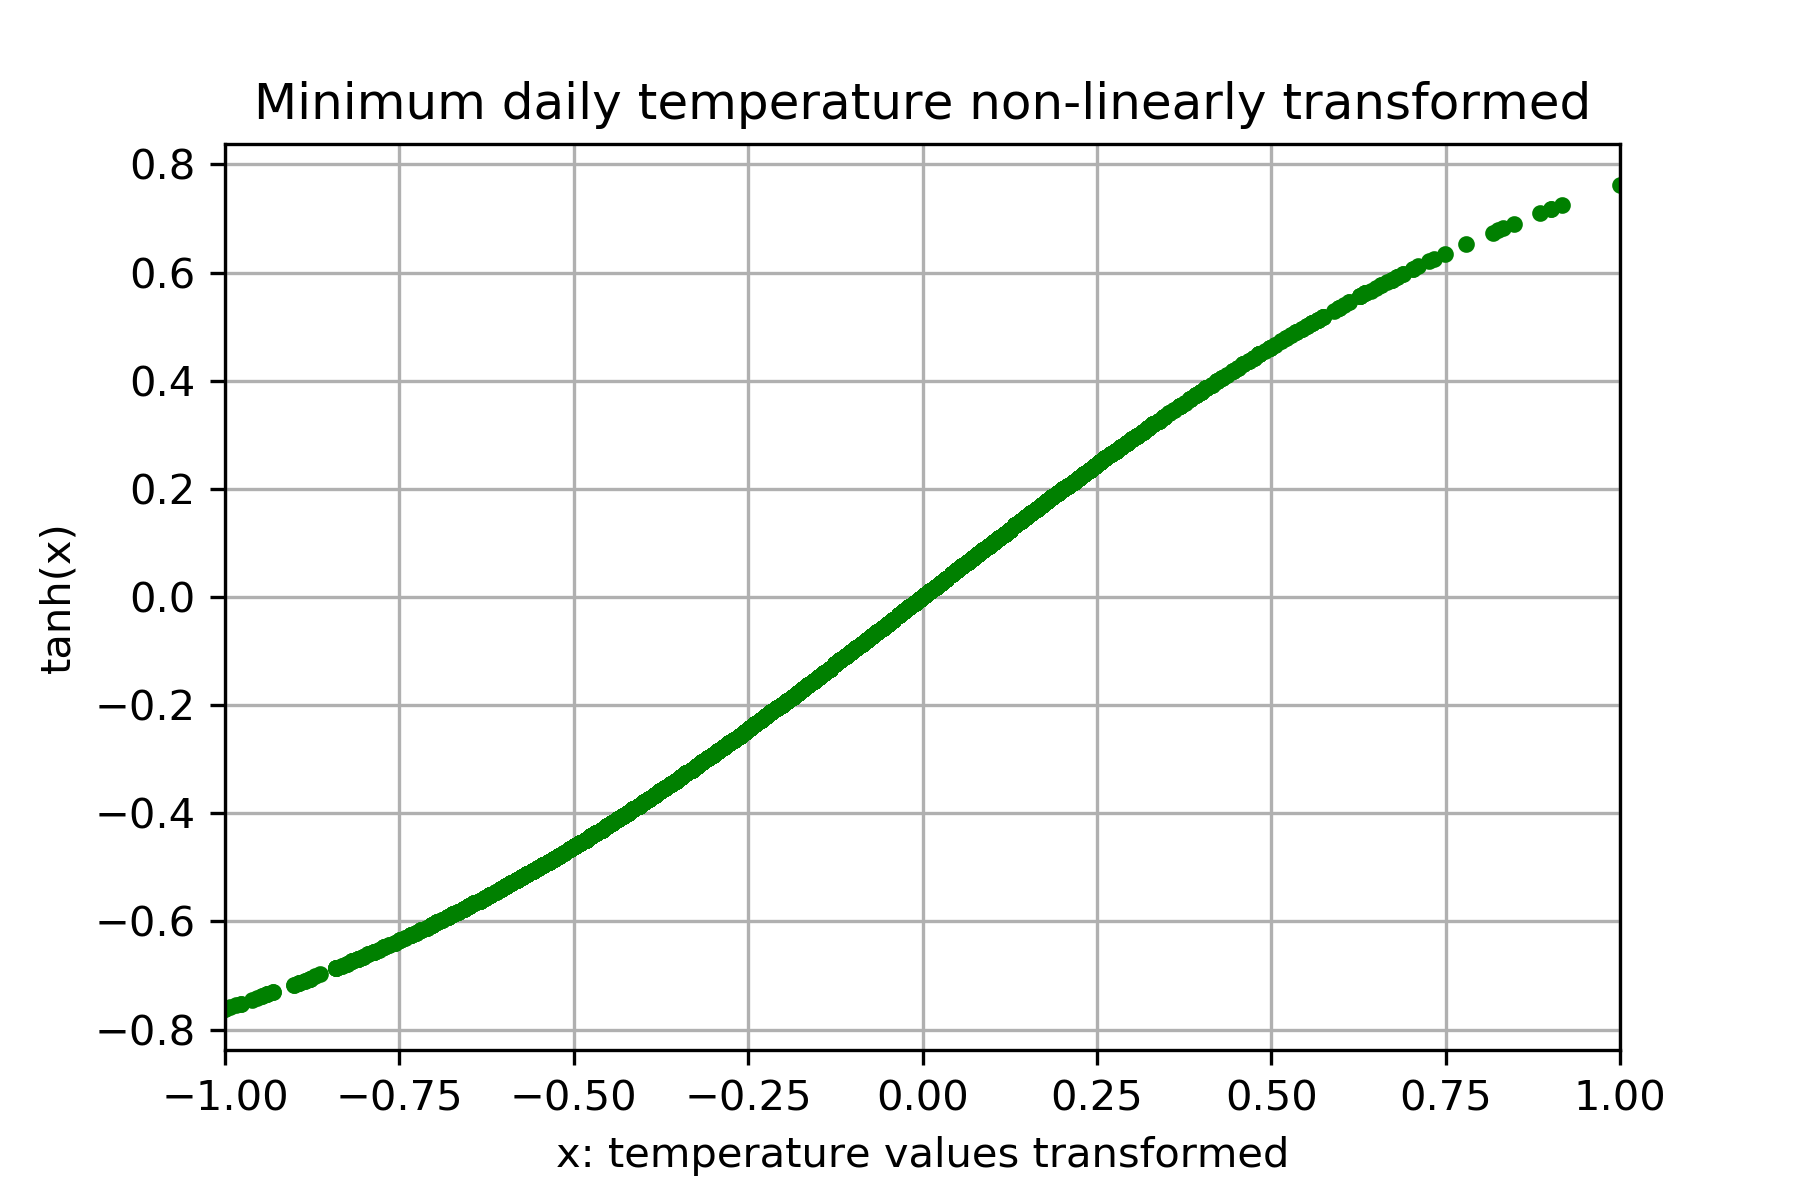
\includegraphics[width=12cm]{figure_3_tanh_dataset}
    \caption{}
    \label{fig:pre-ex2-3}
\end{figure}




\begin{figure}[ht]
    \centering
    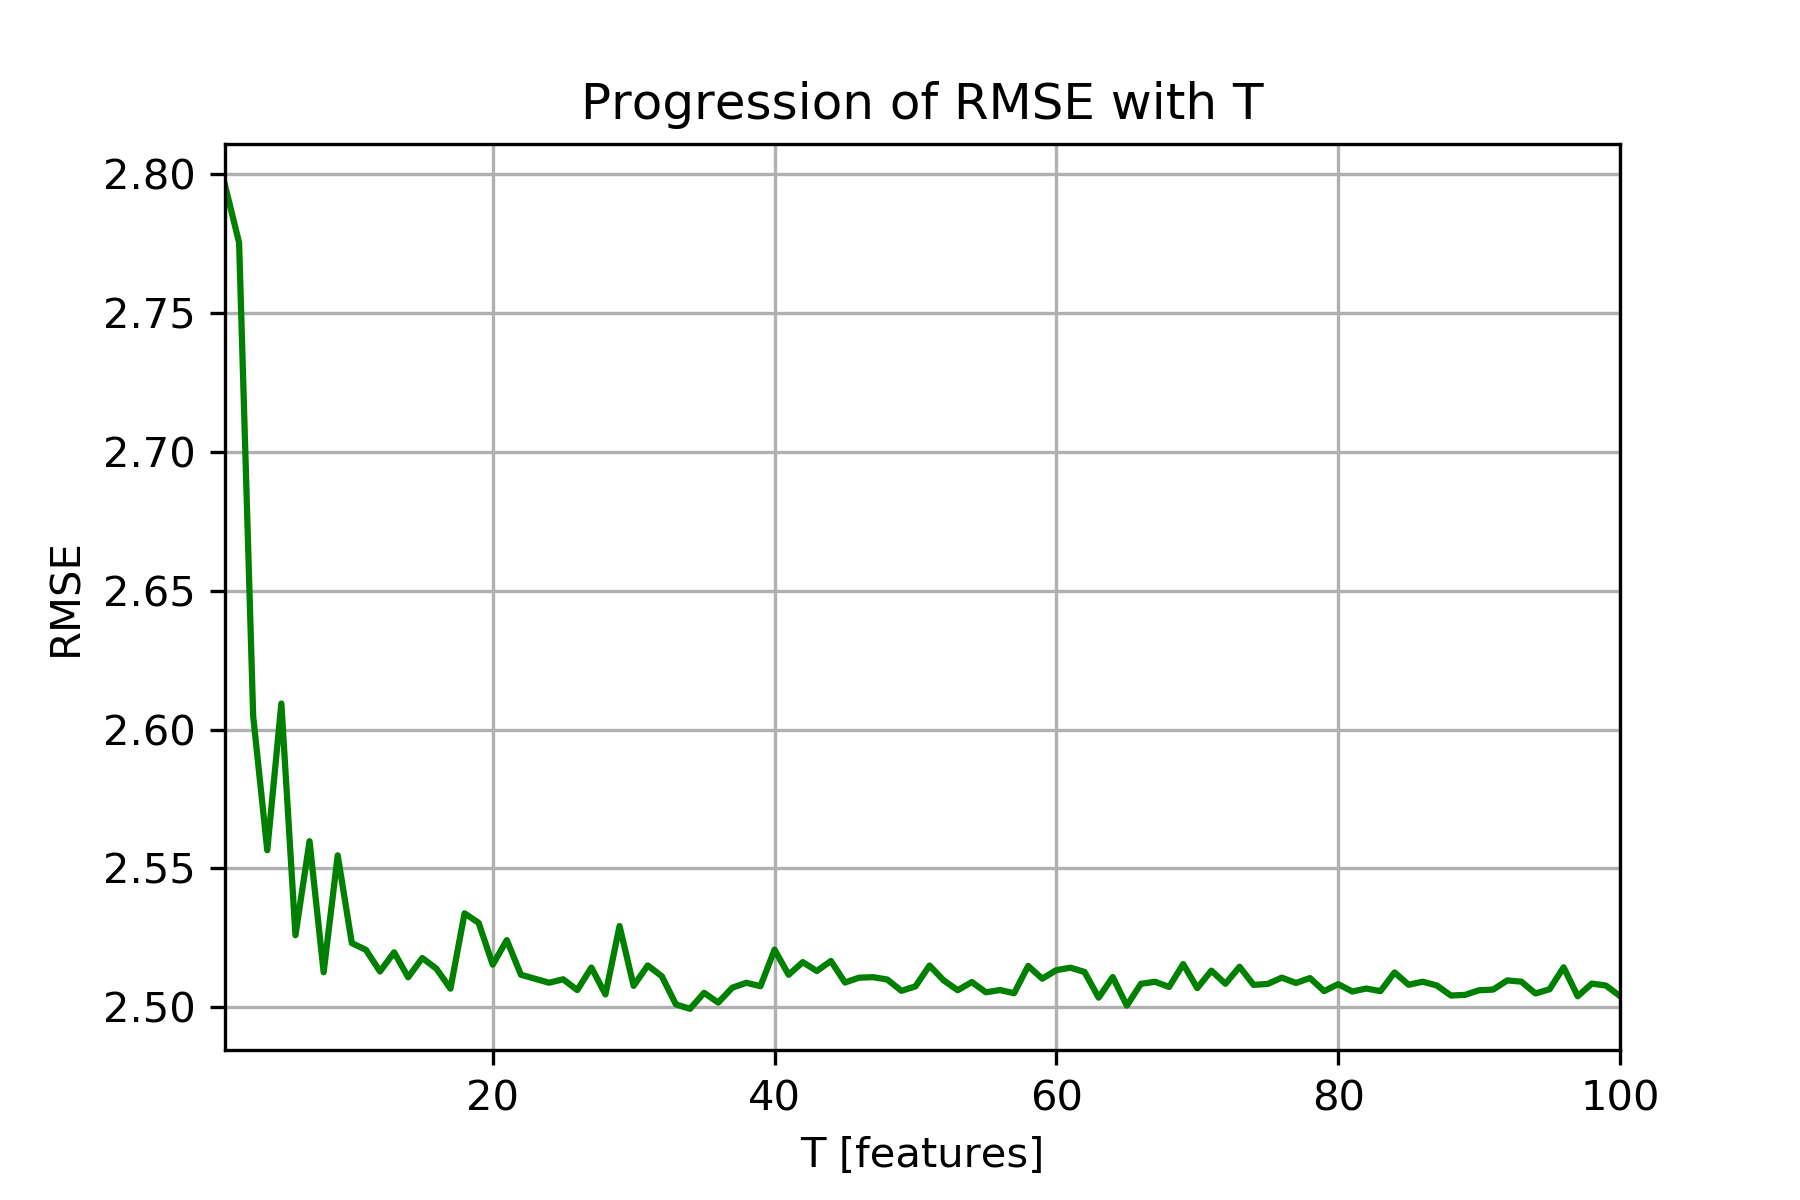
\includegraphics[width=12cm]{figure_1_rmse_with_T}
    \caption{}
    \label{fig:ex2-1}
\end{figure}

\begin{figure}[ht]
    \centering
    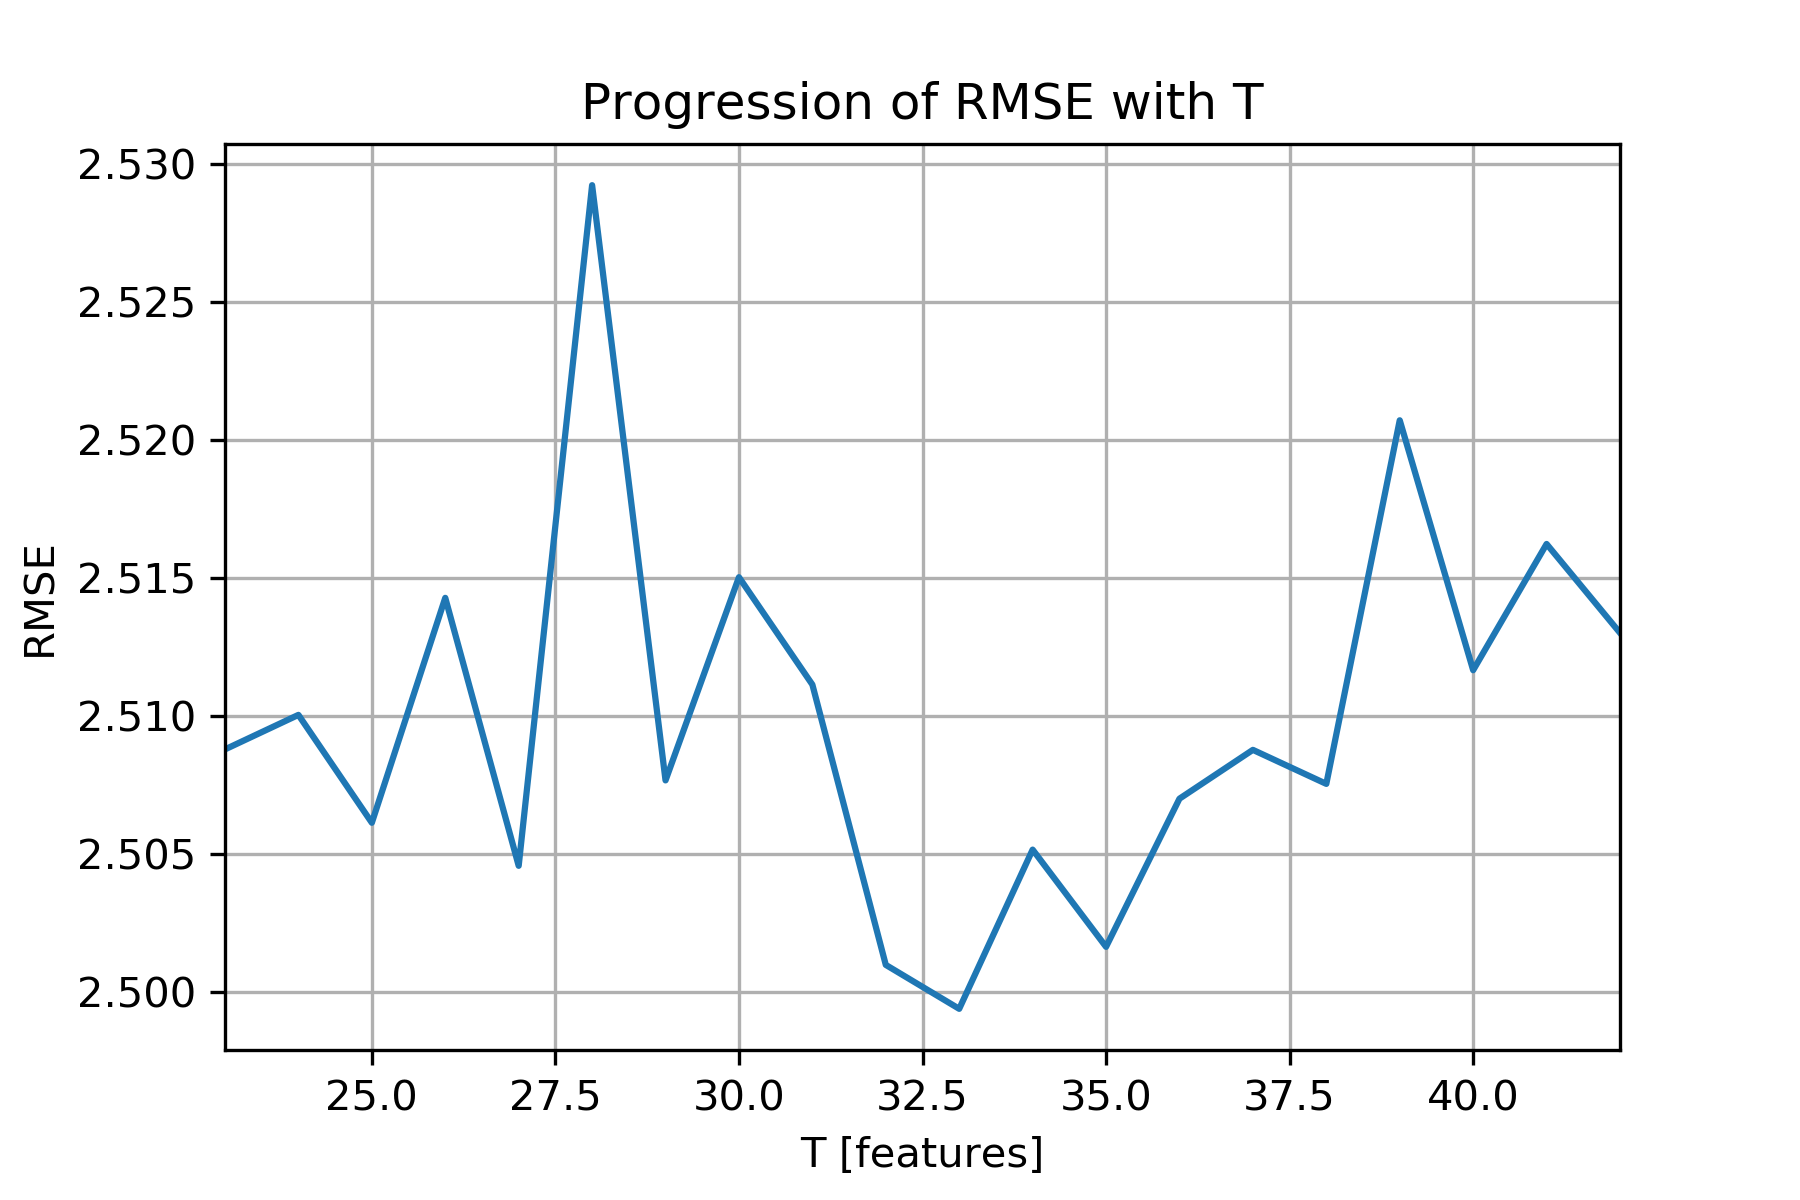
\includegraphics[width=12cm]{figure_2__rmse_with_T_zoom}
    \caption{}
    \label{fig:ex2-2}
\end{figure}

\begin{figure}[ht]
    \centering
    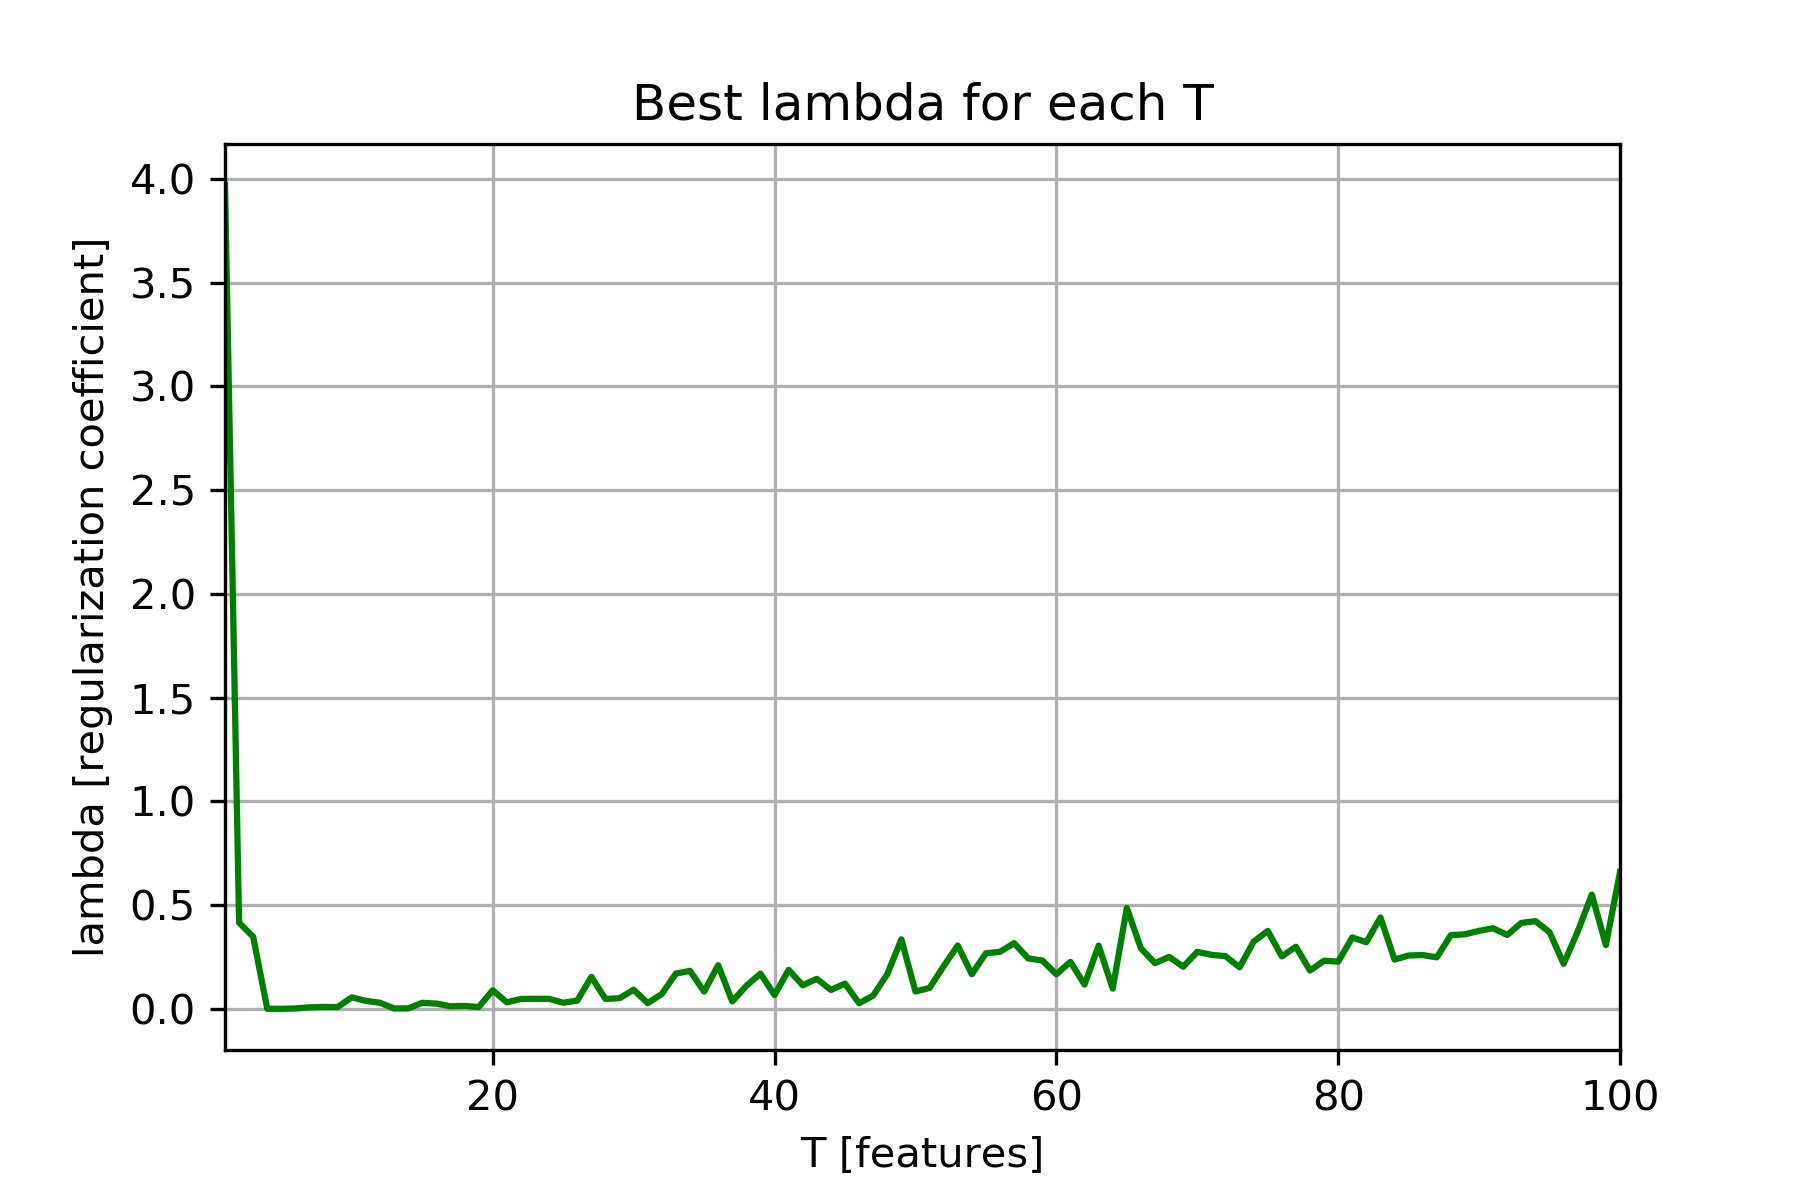
\includegraphics[width=12cm]{figure_3_lambda_with_T}
    \caption{}
    \label{fig:ex2-3}
\end{figure}

\begin{figure}[ht]
    \centering
    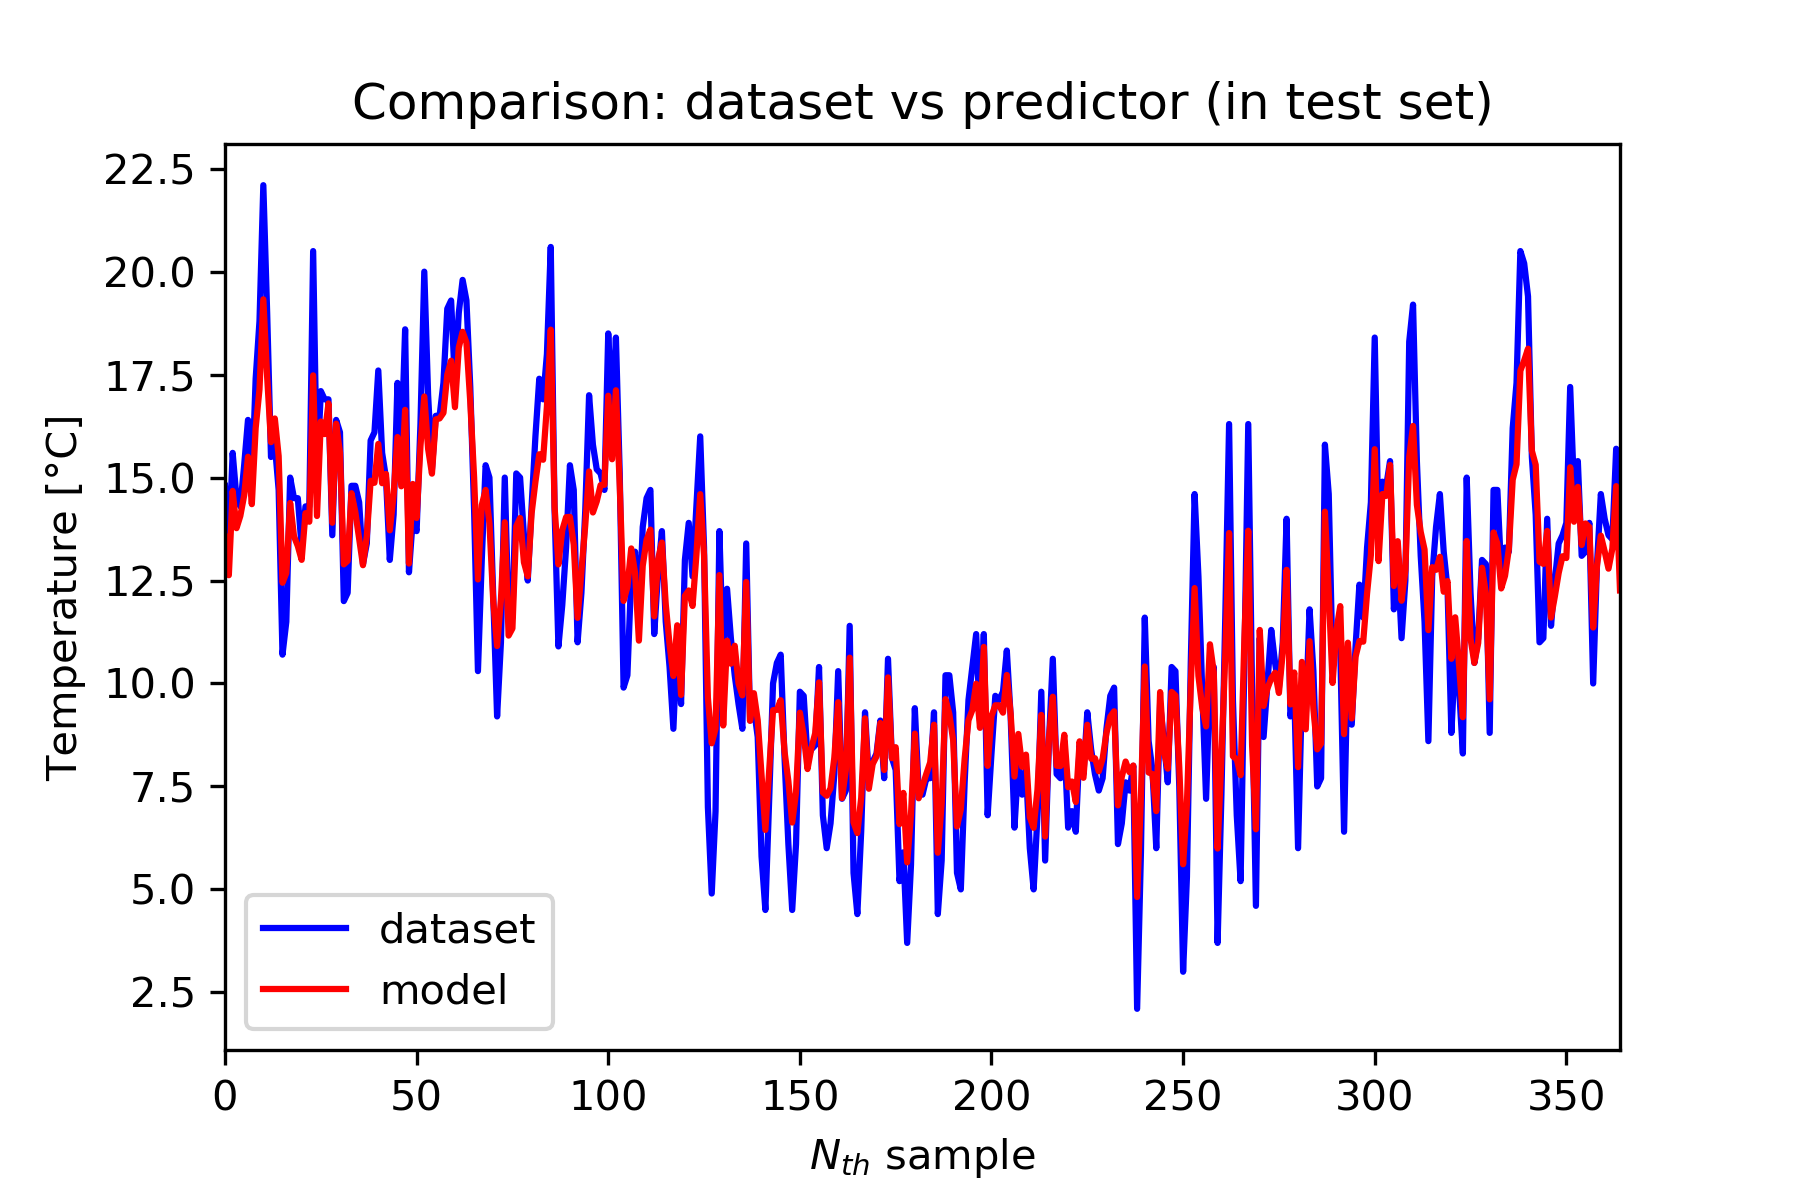
\includegraphics[width=12cm]{figure_4_predictor}
    \caption{}
    \label{fig:ex2-4}
\end{figure}

%==============================
\subsubsection{a) }
%==============================

%==============================
\subsubsection{b) }
%==============================

%==============================
\subsubsection{c) }
%==============================

%=================================================
\end{document}
